%Version 3.1 December 2024
% See section 11 of the User Manual for version history
%
%%%%%%%%%%%%%%%%%%%%%%%%%%%%%%%%%%%%%%%%%%%%%%%%%%%%%%%%%%%%%%%%%%%%%%
%%                                                                 %%
%% Please do not use \input{...} to include other tex files.       %%
%% Submit your LaTeX manuscript as one .tex document.              %%
%%                                                                 %%
%% All additional figures and files should be attached             %%
%% separately and not embedded in the \TeX\ document itself.       %%
%%                                                                 %%
%%%%%%%%%%%%%%%%%%%%%%%%%%%%%%%%%%%%%%%%%%%%%%%%%%%%%%%%%%%%%%%%%%%%%

%%\documentclass[referee,sn-basic]{sn-jnl}% referee option is meant for double line spacing

%%=======================================================%%
%% to print line numbers in the margin use lineno option %%
%%=======================================================%%

%%\documentclass[lineno,pdflatex,sn-basic]{sn-jnl}% Basic Springer Nature Reference Style/Chemistry Reference Style

%%=========================================================================================%%
%% the documentclass is set to pdflatex as default. You can delete it if not appropriate.  %%
%%=========================================================================================%%

%%\documentclass[sn-basic]{sn-jnl}% Basic Springer Nature Reference Style/Chemistry Reference Style

%%Note: the following reference styles support Namedate and Numbered referencing. By default the style follows the most common style. To switch between the options you can add or remove “Numbered” in the optional parenthesis. 
%%The option is available for: sn-basic.bst, sn-chicago.bst%  
 
%%\documentclass[pdflatex,sn-nature]{sn-jnl}% Style for submissions to Nature Portfolio journals
%%\documentclass[pdflatex,sn-basic]{sn-jnl}% Basic Springer Nature Reference Style/Chemistry Reference Style
\documentclass[pdflatex,sn-mathphys-num]{sn-jnl}% Math and Physical Sciences Numbered Reference Style
%%\documentclass[pdflatex,sn-mathphys-ay]{sn-jnl}% Math and Physical Sciences Author Year Reference Style
%%\documentclass[pdflatex,sn-aps]{sn-jnl}% American Physical Society (APS) Reference Style
%%\documentclass[pdflatex,sn-vancouver-num]{sn-jnl}% Vancouver Numbered Reference Style
%%\documentclass[pdflatex,sn-vancouver-ay]{sn-jnl}% Vancouver Author Year Reference Style
%%\documentclass[pdflatex,sn-apa]{sn-jnl}% APA Reference Style
%%\documentclass[pdflatex,sn-chicago]{sn-jnl}% Chicago-based Humanities Reference Style

%%%% Standard Packages
%%<additional latex packages if required can be included here>

\usepackage{graphicx}%
\usepackage{multirow}%
\usepackage{amsmath,amssymb,amsfonts}%
\usepackage{amsthm}%
\usepackage{mathrsfs}%
\usepackage[title]{appendix}%
\usepackage{xcolor}%
\usepackage{textcomp}%
\usepackage{manyfoot}%
\usepackage{booktabs}%
\usepackage{algorithm}%
\usepackage{algorithmicx}%
\usepackage{algpseudocode}%
\usepackage{listings}%
%%%%

%%%%%=============================================================================%%%%
%%%%  Remarks: This template is provided to aid authors with the preparation
%%%%  of original research articles intended for submission to journals published 
%%%%  by Springer Nature. The guidance has been prepared in partnership with 
%%%%  production teams to conform to Springer Nature technical requirements. 
%%%%  Editorial and presentation requirements differ among journal portfolios and 
%%%%  research disciplines. You may find sections in this template are irrelevant 
%%%%  to your work and are empowered to omit any such section if allowed by the 
%%%%  journal you intend to submit to. The submission guidelines and policies 
%%%%  of the journal take precedence. A detailed User Manual is available in the 
%%%%  template package for technical guidance.
%%%%%=============================================================================%%%%

%% as per the requirement new theorem styles can be included as shown below
\theoremstyle{thmstyleone}%
\newtheorem{theorem}{Theorem}%  meant for continuous numbers
%%\newtheorem{theorem}{Theorem}[section]% meant for sectionwise numbers
%% optional argument [theorem] produces theorem numbering sequence instead of independent numbers for Proposition
\newtheorem{proposition}[theorem]{Proposition}% 
%%\newtheorem{proposition}{Proposition}% to get separate numbers for theorem and proposition etc.

\theoremstyle{thmstyletwo}%
\newtheorem{example}{Example}%
\newtheorem{remark}{Remark}%

\theoremstyle{thmstylethree}%
\newtheorem{definition}{Definition}%

\raggedbottom
%%\unnumbered% uncomment this for unnumbered level heads

\begin{document}

\title[Article Title]{Leakage-Free Water Quality Screening: Potability Benchmarks and Rapid Field Assessment Across Indian CPCB Stations}

%%=============================================================%%
%% GivenName	-> \fnm{Joergen W.}
%% Particle	-> \spfx{van der} -> surname prefix
%% FamilyName	-> \sur{Ploeg}
%% Suffix	-> \sfx{IV}
%% \author*[1,2]{\fnm{Joergen W.} \spfx{van der} \sur{Ploeg} 
%%  \sfx{IV}}\email{iauthor@gmail.com}
%%=============================================================%%

\author*[1]{\fnm{Goutham} \sur{P}}\email{csisp260254@cet.ac.in
}

\affil*[1]{\orgdiv{Department of Computer Science and Engineering}, \orgname{College of Engineering Trivandrum}, \orgaddress{\street{Sreekaryam}, \city{Thiruvananthapuram}, \postcode{695016}, \state{Kerala}, \country{India}}}


%%==================================%%
%% Sample for unstructured abstract %%
%%==================================%%

\abstract{Machine learning studies on routine water-quality data frequently report over-optimistic performance due to data leakage during preprocessing. This study establishes a strictly leakage-free framework that encapsulates missing-value imputation, domain-ratio engineering, and standardization inside cross-validation folds. The methodology is evaluated across two distinct settings: a point-of-use drinking-water benchmark of over 3,200 samples, and an applied regional study of 683 lentic stations across 26 Indian States. On the drinking-water benchmark, class-conditional imputation prior to splitting artificially inflated accuracy by 11--13 percentage points. Under a clean protocol, top tree ensembles and kernel classifiers proved statistically indistinguishable, while prioritizing public-health safety by minimizing false-safe errors imposed a steep rejection penalty on genuinely safe water. In the Indian surface-water case study, an 11-feature field-probe model predicting binary CPCB-derived WQI status achieved approximately 87\% pooled out-of-fold accuracy (0.9177--0.9224 ROC-AUC) across unseen states under spatial cross-validation, outperforming linear Logistic Regression (84.92\%--85.36\% accuracy) and matching a deterministic $\text{DO}_{\min} \ge 4.0\text{ mg/L}$ threshold heuristic (87.85\% accuracy) without requiring 5-day biological incubation. These retrospective findings demonstrate that while routine physicochemical sensors have fundamental limits for certifying drinking-water potability, instant field probes offer a promising decision-support tool for rapid surface-water triage pending prospective and external validation.}

%%================================%%
%% Sample for structured abstract %%
%%================================%%

% \abstract{\textbf{Purpose:} The abstract serves both as a general introduction to the topic and as a brief, non-technical summary of the main results and their implications. The abstract must not include subheadings (unless expressly permitted in the journal's Instructions to Authors), equations or citations. As a guide the abstract should not exceed 200 words. Most journals do not set a hard limit however authors are advised to check the author instructions for the journal they are submitting to.
% 
% \textbf{Methods:} The abstract serves both as a general introduction to the topic and as a brief, non-technical summary of the main results and their implications. The abstract must not include subheadings (unless expressly permitted in the journal's Instructions to Authors), equations or citations. As a guide the abstract should not exceed 200 words. Most journals do not set a hard limit however authors are advised to check the author instructions for the journal they are submitting to.
% 
% \textbf{Results:} The abstract serves both as a general introduction to the topic and as a brief, non-technical summary of the main results and their implications. The abstract must not include subheadings (unless expressly permitted in the journal's Instructions to Authors), equations or citations. As a guide the abstract should not exceed 200 words. Most journals do not set a hard limit however authors are advised to check the author instructions for the journal they are submitting to.
% 
% \textbf{Conclusion:} The abstract serves both as a general introduction to the topic and as a brief, non-technical summary of the main results and their implications. The abstract must not include subheadings (unless expressly permitted in the journal's Instructions to Authors), equations or citations. As a guide the abstract should not exceed 200 words. Most journals do not set a hard limit however authors are advised to check the author instructions for the journal they are submitting to.}

\keywords{Water quality screening, Data leakage, Field-probe monitoring, Explainable AI (SHAP), Spatial cross-validation}

%%\pacs[JEL Classification]{D8, H51}

%%\pacs[MSC Classification]{35A01, 65L10, 65L12, 65L20, 65L70}

\maketitle

\section{Introduction}\label{sec1}

Access to reliable, uncontaminated water is a fundamental prerequisite for human health, economic development, and environmental sustainability \cite{unesco2023}. Freshwater resources---encompassing both subsurface aquifers and lentic surface bodies such as lakes, tanks, and ponds---face mounting contamination pressures worldwide. Accelerated industrial discharge, untreated domestic sewage disposal, and intensive agricultural runoff laden with fertilizers and pesticides continuously degrade ambient water reservoirs \cite{akhtar2021,peters2000,rashmi2020}. Water potability and ecological health are determined by complex, non-linear interactions across numerous chemical, physical, and microbiological parameters rather than any isolated property \cite{mccutcheon1992,who2017}. Consequently, statutory water authorities mandate comprehensive laboratory testing to assess water safety. However, standard analytical protocols---most notably the 5-day biochemical oxygen demand ($\text{BOD}_5$) incubation and multi-tube fermentation for fecal and total coliforms---impose unavoidable multi-day delays. These operational bottlenecks impede rapid containment and prevent environmental officers from executing on-site triage when contamination events emerge.

To overcome these latency constraints, data-driven computational techniques have emerged as a promising decision-support paradigm. Supervised machine learning (ML) models aim to emulate expert diagnostic assessment by learning functional mappings between readily measurable physicochemical indicators and overall water safety. In a recent benchmark study, Rachid et al. \cite{rachid2025} evaluated Random Forest (RF) and Support Vector Machine (SVM) models on the widely referenced Kaggle drinking-water potability dataset \cite{kadiwal2020}, reporting $70\%$ accuracy and $0.75$ receiver operating characteristic area under the curve (ROC-AUC) for RF after dropping incomplete records and undersampling to balance classes. Earlier investigations on related benchmarks similarly reported competitive predictive performance using gradient boosting, decision trees, and neural architectures \cite{ghosh2023,kaddoura2022,ahmed2019,bui2020,aldhyani2020}.

Despite extensive academic interest, a rigorous audit of the contemporary water-quality ML literature exposes five fundamental methodological and operational limitations:
\begin{enumerate}
    \item \textit{Pervasive Data Leakage:} A substantial portion of published studies reporting accuracies above $80$--$90\%$ apply missing-value imputation (particularly class-conditional mean imputation) or feature normalization across the full dataset prior to train--test partitioning \cite{kaufman2012,kapoor2023}. This leaks target and distribution properties from evaluation sets into training routines, generating severely inflated, irreproducible performance metrics.
    \item \textit{Discard-Driven Sample Bias:} Rather than evaluating missing-data imputation inside cross-validation, common workflows discard all observations with missing values. In typical monitoring datasets, this practice eliminates over one-third of available historical data, altering empirical feature correlations and reducing real-world representativeness.
    \item \textit{Inverted Public-Health Risk Framing:} Standard machine learning workflows predominantly focus on overall accuracy or positive-class (potable) precision. In water safety screening, however, the catastrophic public-health hazard is the False-Safe error---classifying unsafe, non-potable water as potable. The primary safety metric is therefore Unsafe-Water Recall (Specificity), yet it is frequently omitted in model selection.
    \item \textit{Uncalibrated Probability Scores and Unstated Rejection Costs:} Tree ensemble models trained with class-balancing heuristics yield distorted score distributions rather than calibrated Bayesian posterior probabilities. While tightening classification thresholds can suppress false-safe predictions, it invariably increases false rejections of safe water. The practical operational cost of this trade-off is almost universally unquantified in existing literature.
    \item \textit{Spatial Non-Independence in Surface-Water Monitoring:} In regional surface-water quality modeling, monitoring stations situated within the same watershed or administrative state share correlated hydrological, climatic, and wastewater management profiles, exhibiting marked spatial autocorrelation \cite{legendre1993,roberts2017,ploton2020}. Evaluating models using naive random splits fails to test true geographical transferability, leading to over-optimistic performance claims on unmonitored water bodies \cite{meyer2018}.
\end{enumerate}

To systematically address these vulnerabilities, this study introduces an end-to-end, strictly leakage-free machine learning framework evaluated across two distinct, complementary experimental settings. First, we carry out a rigorous methodological audit on the complete Kaggle point-of-use drinking-water benchmark ($N = 3,276$). We retain all records by encapsulating multivariate iterative imputation, domain-ratio feature engineering, and standardization inside cross-validation folds. Using Repeated Stratified $5 \times 3$ cross-validation paired with the Nadeau--Bengio \cite{nadeau2003} corrected resampled $t$-test, we establish whether hyperparameter tuning and complex imputation deliver statistically meaningful gains over simple baselines, quantify the trade-off of frozen safety-first thresholds under isotonic probability calibration, and empirically demonstrate the magnitude of performance inflation caused by target leakage.

Second, we extend this leak-free methodology to an applied regional case study utilizing official monitoring records from the Central Pollution Control Board (CPCB) National Water Quality Monitoring Programme (NWMP) across 683 lentic stations in 26 Indian States and Union Territories \cite{cpcb2024}. Recognizing that ambient surface water evaluated under a Water Quality Index (WQI) represents a distinct operational task from point-of-use tap potability (governed in India by BIS IS 10500:2012), we examine whether an 11-feature Instant Field-Probe model---relying exclusively on on-site sensor measurements of temperature, dissolved oxygen, pH, electrical conductivity, and nitrate---can triage degraded surface waters across unseen states without waiting 5 days for laboratory $\text{BOD}_5$ and coliform assays. Using spatial 5-fold \texttt{GroupKFold} and 26-state Leave-One-State-Out cross-validation on identical folds, we benchmark this field probe against linear formula-subset baselines and single-sensor heuristics.

By bridging methodological audit rigor with real-world regional catchment screening, this work provides environmental practitioners, data scientists, and water utilities with an honest, reproducible baseline for deploying machine learning responsibly in water quality monitoring.

\section{Related Work}\label{sec2}

\subsection{Machine Learning in Drinking-Water Potability Assessment}\label{subsec2_1}
The application of supervised machine learning to drinking-water potability prediction has expanded rapidly as researchers seek to replace or complement labor-intensive physical testing. Early investigations on physicochemical benchmarks explored standard classification algorithms to map routine sensor readings directly to potability labels. Kaddoura \cite{kaddoura2022} evaluated multiple supervised models on water-quality records and demonstrated that Support Vector Machines (SVM) and $k$-Nearest Neighbors (KNN) attained competitive predictive capability in terms of F1-score and area under the ROC curve. In a multi-model comparative assessment, Ghosh et al. \cite{ghosh2023} applied Gaussian Naive Bayes, Bernoulli Naive Bayes, Decision Trees, SVM, KNN, XGBoost, and Random Forest (RF) to predict water safety, concluding that ensemble decision trees achieved the highest accuracy ($78.96\%$) while kernel methods yielded lower precision ($68.29\%$).

Building upon these findings, Rachid et al. \cite{rachid2025} recently investigated the comparative efficiency of RF and SVM on the public Kaggle drinking-water dataset. To address class imbalance and data quality issues, their pipeline eliminated all records containing missing entries and applied random undersampling to balance 811 potable instances with 811 non-potable instances ($N = 1,622$). Evaluating across a 70/20/10 train-validation-test partition and 5-fold cross-validation, their study reported $70\%$ test accuracy and $0.75$ ROC-AUC for RF, whereas SVM degraded to $48\%$ accuracy and $0.47$ ROC-AUC.

Beyond purely chemical parameters, machine learning has also been explored for estimating microbiological contamination in source water. Sokolova et al. \cite{sokolova2022} developed predictive models using historical hydrometeorological records and routine parameters to forecast \textit{Escherichia coli} levels in drinking-water intakes, identifying RF as the most robust predictor across changing environmental conditions. Similarly, Mohammed et al. \cite{mohammed2017} utilized RF classifiers trained on raw water conductivity, pH, turbidity, color, and seasonal indicators to anticipate fecal contamination in Bergen, Norway, illustrating the potential of tree-based ensembles for early contamination alert systems.

\subsection{Machine Learning in Ambient Surface Water and Catchment Monitoring}\label{subsec2_2}
In parallel with point-of-use drinking-water studies, artificial intelligence has been deployed extensively for ambient surface-water monitoring and Water Quality Index (WQI) estimation \cite{horton1965,brown1970,tyagi2013,abbasi2012}. Haghiabi et al. \cite{haghiabi2018} evaluated Artificial Neural Networks (ANN), Group Method of Data Handling (GMDH), and SVM to predict water quality components along the Tireh River in southwestern Iran, finding that SVM projected non-linear chemical interactions with higher fidelity than traditional regressors. Azrour et al. \cite{azrour2022} assessed ML algorithms for surface-water classification, identifying neural networks as the most capable architecture for approximating complex non-linear WQI aggregations.

In the Indian context, Ainapure et al. \cite{ainapure2023} examined supervised machine learning algorithms to assess the potability and pollution status of river systems, emphasizing the regional importance of rapid water quality triage for vulnerable populations. Broad synthesis reviews by Zhu et al. \cite{zhu2022}, Yan et al. \cite{yan2024}, and Rajaee et al. \cite{rajaee2019} surveyed extensive years of literature in aquatic ML prediction, concluding that while ensemble trees, gradient boosting, and deep neural networks consistently achieve high reported performance, their operational value in real-world deployments is severely compromised by noisy sensor readings, unresolved missing data, arbitrary class-boundary definitions, and a failure to evaluate spatial generalization across distinct river basins.

\subsection{Methodological Deficits in Existing Literature}\label{subsec2_3}
Despite the proliferation of water-quality ML papers, a rigorous examination of published pipelines reveals critical methodological flaws that undermine their scientific validity:
\begin{enumerate}
    \item \textit{Target and Preprocessing Leakage:} Many published studies reporting $>80\%$ accuracy fit imputers, scalers, or feature selection routines across the entire dataset before splitting. In particular, class-conditional mean imputation---filling missing features with the mean of their target class---directly injects the label into the features, generating artificial performance that collapses on real unseen data \cite{vabalas2019,kapoor2023,kaufman2012}.
    \item \textit{Arbitrary Data Pruning:} Eliminating incomplete records (as done in Rachid et al. \cite{rachid2025}) discards over $40\%$ of available monitoring data, masking real-world sensor dropout patterns and altering empirical feature distributions.
    \item \textit{Inattention to False-Safe Public-Health Risk:} Most studies report overall accuracy or positive-class precision, ignoring that the primary public-health disaster is classifying contaminated water as safe. The critical safety metric is Unsafe-Water Recall (Specificity), which is rarely reported or prioritized.
    \item \textit{Invalid Statistical Comparisons:} Studies comparing multiple cross-validation folds frequently apply standard paired $t$-tests. Because repeated cross-validation folds share training instances, standard tests violate independence assumptions and produce anti-conservative, falsely significant $p$-values unless corrected \cite{nadeau2003}.
    \item \textit{Spatial Autocorrelation Ignored:} Surface-water monitoring stations within the same state or river basin share underlying catchments and regulatory practices. Random train-test splits allow neighboring stations to appear in both sets, overestimating performance on genuinely unmonitored geographic regions \cite{legendre1993,roberts2017,ploton2020}.
\end{enumerate}

This study directly addresses each of these five deficits through a leak-free pipeline, Nadeau--Bengio hypothesis testing, public-health risk thresholding, and state-grouped spatial cross-validation.
\begin{table}[t]
\caption{Summary of related machine learning studies in water quality assessment and identified research gaps}\label{tab_lit_review}%
\footnotesize
\begin{tabular}{@{}p{0.17\textwidth}p{0.15\textwidth}p{0.17\textwidth}p{0.17\textwidth}p{0.22\textwidth}@{}}
\toprule
Study & Scope & Models & Reported Result & Key Limitations\footnotemark[1] \\
\midrule
Kaddoura \cite{kaddoura2022} & Drinking water & SVM, KNN & High F1 \& ROC-AUC & Single split; no data leakage audit. \\
Mohammed et al. \cite{mohammed2017} & Raw water (Norway) & Random Forest & Accurate fecal prediction & Focused only on bacteria; no missing data study. \\
Ghosh et al. \cite{ghosh2023} & Water potability & RF, SVM, XGBoost & RF: 78.96\% Acc & Standard accuracy focus; unverified leakage. \\
Rachid et al. \cite{rachid2025}\footnotemark[2] & Kaggle ($N=1,622$) & Random Forest, SVM & RF: 70\% Acc (0.75 AUC) & Discarded missing rows; undersampled; no spatial CV. \\
Azrour et al. \cite{azrour2022} & Surface water WQI & ANN, ML models & High WQI correlation & Evaluated on random split; ignores catchment clustering. \\
\botrule
\end{tabular}
\footnotetext[1]{Key limitations identified across prior literature that motivate the methodological design of the present study.}
\footnotetext[2]{Base comparison study published in \textit{Environmental Challenges} (Elsevier, 2025).}
\end{table}
\\
\section{Problem Statement}\label{sec3}

Water quality assessment via machine learning faces two critical bottlenecks across drinking-water certification and ambient environmental monitoring:
\begin{enumerate}
    \item \textit{Methodological Deficits in Drinking-Water Benchmarks:} Published models predicting drinking-water potability from routine physicochemical parameters frequently suffer from target leakage caused by imputing missing values or scaling features across the entire dataset before splitting \cite{kaufman2012,kapoor2023}. This creates artificial accuracy spikes that fail in real-world deployment. Conversely, discarding incomplete records eliminates over $40\%$ of available monitoring data. Furthermore, conventional workflows optimize overall accuracy while ignoring the primary public-health hazard: the False-Safe error (passing contaminated water as potable) \cite{elkan2001,he2009}. Because class-balanced models output uncalibrated scores, the operational cost of tightening decision thresholds---specifically the resulting rejection rate of genuinely safe water---remains unquantified under cost-sensitive frameworks \cite{he2009}.
    \item \textit{Operational Delays in Surface-Water Screening:} In ambient surface-water monitoring across lakes, ponds, and tanks, regulatory Water Quality Index (WQI) grading \cite{brown1970,tyagi2013} requires 5-day biochemical oxygen demand ($\text{BOD}_5$) and coliform bacteria incubation. This 5-day laboratory delay prevents rapid on-site detection of acute pollution events. Moreover, because stations within the same state share catchments and management practices, evaluating models on naive random splits overestimates performance across unseen regions due to spatial autocorrelation \cite{roberts2017,ploton2020}.
\end{enumerate}

To address these challenges, this study formulates three concrete objectives:
\begin{itemize}
    \item Establish a strictly leakage-free pipeline where all imputation, ratio engineering, and scaling parameters are fitted exclusively within active training folds ($\boldsymbol{\theta} = \mathcal{T}(\mathcal{D}_{\text{train}})$);
    \item Evaluate safety-first operating thresholds under calibrated probabilities, explicitly quantifying the trade-off between suppressing false-safe errors and rejecting safe water; and
    \item Validate an 11-feature instant field-probe model under state-grouped (\texttt{GroupKFold}) and Leave-One-State-Out (\texttt{LeaveOneGroupOut}) spatial cross-validation to assess whether rapid on-site triage is feasible without 5-day laboratory assays.
\end{itemize}

\section{Materials and Methods}\label{sec4}
This section details the experimental framework developed for leak-free water quality classification. We introduce the drinking-water and surface-water datasets, formalize the encapsulated preprocessing pipeline that prevents data contamination, and specify the model training, probability calibration, and spatial validation protocols.
\subsection{Datasets}\label{subsec4_1}

Two public datasets representing distinct water-monitoring regimes are analyzed in this study:

\subsubsection{Point-of-Use Drinking-Water Benchmark (Kaggle Dataset)}\label{subsubsec4_1_1}
The benchmark dataset comprises $N = 3,276$ point-of-use water quality records with nine physicochemical features \cite{kadiwal2020} (\texttt{ph}, \texttt{Hardness}, \texttt{Solids}, \texttt{Chloramines}, \texttt{Sulfate}, \texttt{Conductivity}, \texttt{Organic\_carbon}, \texttt{Trihalomethanes}, and \texttt{Turbidity}) and a binary potability label ($1,998$ non-potable [$60.99\%$]; $1,278$ potable [$39.01\%$]). It contains zero duplicate rows. Missing values occur across three features: \texttt{Sulfate} ($781$, $23.84\%$), \texttt{ph} ($491$, $14.99\%$), and \texttt{Trihalomethanes} ($162$, $4.95\%$), totaling $1,434$ missing entries ($4.86\%$ of all feature values). Monitored parameters and regulatory reference baselines are summarized in Table~\ref{tab_who}.
\begin{table}[t]
\caption{Physicochemical parameters in the drinking-water benchmark ($N = 3,276$) and international reference context \cite{who2017,rachid2025}.}\label{tab_who}%
\begin{tabular}{@{}p{0.22\textwidth}p{0.18\textwidth}p{0.52\textwidth}@{}}
\toprule
Parameter & Unit & WHO / EPA Reference Context\footnotemark[1] \\
\midrule
pH & pH units & $6.5$--$8.5$ (operational range) \\
Chloramines & $\text{mg/L}$ & $\le 4.0\text{ mg/L}$ \\
Sulfate & $\text{mg/L}$ & $250\text{ mg/L}$ \\
Organic carbon (TOC) & $\text{mg/L}$ & $< 2.0\text{ mg/L}$ (treated water) \\
Trihalomethanes & $\mu\text{g/L}$ & $\le 80\text{ }\mu\text{g/L}$ \\
Hardness & $\text{mg/L}$ & $120$--$180\text{ mg/L}$ \\
Solids (TDS) & $\text{mg/L}$ & $500$--$1000\text{ mg/L}$ (palatability) \\
Conductivity & $\mu\text{S/cm}$ & $500$--$1500\text{ }\mu\text{S/cm}$ \\
Turbidity & NTU & $\le 5\text{ NTU}$ \\
\botrule
\end{tabular}
\footnotetext[1]{Reference ranges compiled from WHO Guidelines for Drinking-water Quality (4th ed.) \cite{who2017}, US EPA standards \cite{usepa2018}, and Indian Standard IS 10500:2012 \cite{bis2012}.}
\end{table}

\subsubsection{Indian CPCB Ambient Surface-Water Dataset (Regional Case Study)}\label{subsubsec4_1_2}
The regional case study examines $N = 683$ lentic surface-water monitoring stations across 26 Indian States and Union Territories from the processed CPCB-NWMP Mendeley Data repository (v2, 2024) \cite{cpcb2024}, encompassing $488$ lakes ($71.45\%$), $98$ tanks ($14.35\%$), and $97$ ponds ($14.20\%$). All $683$ records correspond to unique \texttt{station\_id} entries with zero missing values and zero duplicate records. Each station records minimum and maximum values across eight physicochemical and microbiological parameters (16 raw features; Table~\ref{tab_cpcb}); individual sampling dates and timestamps are not included in this processed release. Regulatory targets follow the pre-assigned CPCB Water Quality Index (WQI) designations: a 4-class classification (\texttt{Excellent}: $156$, \texttt{Good}: $213$, \texttt{Poor}: $142$, \texttt{Very Poor}: $172$) and a binary screening mapping (\texttt{Acceptable = 1} $\equiv \{\texttt{Excellent}, \texttt{Good}\}$, $n = 369$ [$54.03\%$]; \texttt{Degraded = 0} $\equiv \{\texttt{Poor}, \texttt{Very Poor}\}$, $n = 314$ [$45.97\%$]). As CPCB monitors ambient surface waters rather than treated tap water, this cohort serves strictly as a regional surface-water quality assessment.

\begin{table}[t]
\caption{Monitored parameters in the Indian CPCB lentic dataset ($N = 683$) categorized by field sensing feasibility \cite{cpcb2024}.}\label{tab_cpcb}%
\begin{tabular}{@{}p{0.28\textwidth}p{0.52\textwidth}p{0.14\textwidth}@{}}
\toprule
Parameter & Features (Min \& Max) & Unit \\
\midrule
\multicolumn{3}{@{}l}{\textbf{Instant Field-Probe Suite (11 Features --- Rapid On-Site Triage)\footnotemark[1]}} \\
Temperature & \texttt{Temp\_min}, \texttt{Temp\_max} & $^\circ\text{C}$ \\
Dissolved Oxygen & \texttt{DO\_min}, \texttt{DO\_max} & $\text{mg/L}$ \\
pH & \texttt{pH\_min}, \texttt{pH\_max} & pH units \\
Conductivity & \texttt{EC\_min}, \texttt{EC\_max} & $\mu\text{S/cm}$ \\
Nitrate & \texttt{Nitrate\_min}, \texttt{Nitrate\_max} & $\text{mg/L}$ \\
pH-to-EC Ratio & \texttt{pH\_EC\_ratio} & --- \\
\midrule
\multicolumn{3}{@{}l}{\textbf{Laboratory Assays (Excluded from Field Probe, Used in 18-Feature Suite)\footnotemark[2]}} \\
Biochemical Oxygen Demand & \texttt{BOD\_min}, \texttt{BOD\_max} & $\text{mg/L}$ \\
Fecal Coliforms & \texttt{FC\_min}, \texttt{FC\_max} & $\text{MPN}/100\text{mL}$ \\
Total Coliforms & \texttt{TC\_min}, \texttt{TC\_max} & $\text{MPN}/100\text{mL}$ \\
DO-to-BOD Ratio & \texttt{DO\_BOD\_ratio} & --- \\
\botrule
\end{tabular}
\footnotetext[1]{Instant field-probe suite delivers immediate classification within minutes without lab incubation delays.}
\footnotetext[2]{Standard laboratory assays require up to 5 days incubation, causing significant turnaround latency in field screening.}
\end{table}

\subsection{Leak-Free Preprocessing and Feature Pipeline}\label{subsec4_2}

To ensure zero train--test contamination during validation and evaluation, a strict data partitioning and encapsulation protocol is enforced. For the point-of-use drinking-water benchmark ($N = 3,276$), a two-stage stratified partition with a fixed seed allocates $70\%$ of samples to training ($\mathcal{D}_{\text{train}}$, $n = 2,293$), $15\%$ to validation ($\mathcal{D}_{\text{val}}$, $n = 491$), and $15\%$ to an immutable holdout test partition ($\mathcal{D}_{\text{test}}$, $n = 492$). The holdout partition is strictly sequestered and evaluated only once on the finalized model pipelines.

All transformation steps are encapsulated within an end-to-end \texttt{sklearn.pipeline.Pipeline} architecture \cite{pedregosa2011} that prevents data snooping:
\begin{enumerate}
    \item \textbf{Multivariate Iterative Imputation:} Missing feature values ($1,434$ cells across \texttt{Sulfate}, \texttt{ph}, and \texttt{Trihalomethanes}) are imputed using \texttt{scikit-learn}'s \texttt{IterativeImputer} (inspired by Multivariate Imputation by Chained Equations, MICE \cite{vanbuuren2011,little2019}) with an \texttt{ExtraTreesRegressor} estimator ($50$ trees, maximum depth of $10$, $\text{max\_iter} = 10$). Imputation models are fit exclusively on the active training folds and applied out-of-fold to validation and test records, completely avoiding target-stratified mean imputation leakage.
    \item \textbf{Domain Feature Engineering:} Through a parallel \texttt{FeatureUnion}, an interaction ratio capturing acid--base mineralization equilibrium is constructed:
    \begin{equation}
        \text{ph\_sulfate\_ratio} = \frac{\text{pH}}{\max(|\text{Sulfate}|, 10^{-6})}
        \label{eq:ratio}
    \end{equation}
    evaluated via a zero-guarded reciprocal transformer and a degree-2 \texttt{PolynomialFeatures(interaction\_only=True)} step that retains only the cross-product $\text{pH} \times (1/\text{Sulfate})$, producing $d = 10$ input features ($9$ raw features plus \texttt{ph\_sulfate\_ratio}).
    \item \textbf{Z-Score Standardization:} All $10$ features are centered to zero mean and scaled to unit variance using \texttt{StandardScaler}, with empirical scaling parameters $\boldsymbol{\mu}_{\text{train}}$ and $\boldsymbol{\sigma}_{\text{train}}$ calculated solely from active training partitions.
\end{enumerate}

For the Indian CPCB lentic dataset ($N = 683$), preprocessing evaluates two distinct operational configurations across $70\%/15\%/15\%$ stratified partitions ($n_{\text{train}} = 478$, $n_{\text{val}} = 102$, $n_{\text{test}} = 103$) as well as full-cohort spatial cross-validation:
\begin{itemize}
    \item \textbf{Full Laboratory Suite (18 Features):} Encapsulates all 16 observed min/max parameters alongside two derived equilibrium indices: $\text{DO\_BOD\_ratio} = \text{DO}_{\min} / (\text{BOD}_{\max} + 10^{-6})$ and $\text{pH\_EC\_ratio} = \text{pH}_{\max} / (\text{EC}_{\max} + 10^{-6})$. Because ground-truth WQI labels are computed deterministically from these identical inputs, this suite quantifies algorithmic \textit{formula-emulation fidelity}.
    \item \textbf{Instant Field-Probe Suite (11 Features):} Excludes the delayed 5-day laboratory incubation assays (\texttt{BOD\_min}, \texttt{BOD\_max}) and microbiological cultures (\texttt{FC\_min}, \texttt{FC\_max}, \texttt{TC\_min}, \texttt{TC\_max}). It retains exclusively the 10 real-time field-sensor parameters (\texttt{Temp}, \texttt{DO}, \texttt{pH}, \texttt{EC}, \texttt{Nitrate} min/max) and \texttt{pH\_EC\_ratio}, representing a practical on-site screening configuration with partial-formula overlap.
\end{itemize}


\subsection{Classification Algorithms and Baseline Formulations}\label{subsec4_3}

Six supervised classification architectures representing diverse inductive biases are benchmarked under identical preprocessing pipelines:

\begin{enumerate}
    \item \textbf{Proposed Hyperparameter-Tuned Random Forest:} An ensemble of randomized decision trees \cite{breiman2001} parameterized to mitigate high feature correlation and moderate sample size while maximizing margin separation.
    \item \textbf{Plain Random Forest Baseline:} A standard unpruned ensemble with $300$ estimators \cite{breiman2001} and default split criteria, providing an untuned ensemble baseline.
    \item \textbf{Support Vector Machine (SVM):} Employs a non-linear Radial Basis Function (RBF) kernel \cite{cortes1995} (RBF) kernel $K(\mathbf{x}_i, \mathbf{x}_j) = \exp(-\gamma \|\mathbf{x}_i - \mathbf{x}_j\|^2)$ with Platt scaling calibrated to yield posterior probabilities $P(Y=1 \mid \mathbf{x})$.
    \item \textbf{Logistic Regression:} An $\ell_2$-regularized linear model \cite{cox1958} optimized via the L-BFGS quasi-Newton solver \cite{liu1989} ($2000$ iterations) establishing the linear boundary performance ceiling.
    \item \textbf{Decision Tree Classifier (CART):} A single interpretable orthogonal recursive partitioning tree constrained to a maximum depth of $8$ and a minimum leaf size of $5$ samples \cite{breiman1984}.
    \item \textbf{$k$-Nearest Neighbors ($k$-NN):} A non-parametric instance-based classifier \cite{cover1967} utilizing Euclidean distance metrics with distance-weighted voting across $k = 9$ neighbors.
\end{enumerate}

To counter the empirical class imbalance in the drinking-water benchmark ($60.99\%$ non-potable vs. $39.01\%$ potable), cost-sensitive loss weighting is applied across all eligible classifiers using the inverse frequency formulation \cite{he2009}:
\begin{equation}
    w_c = \frac{N}{2 \cdot N_c}, \quad c \in \{0, 1\}
    \label{eq:class_weight}
\end{equation}
assigning weights $w_0 \approx 0.820$ and $w_1 \approx 1.282$ to penalize minority misclassifications without distorting underlying sample density via synthetic oversampling.


\subsection{Hyperparameter Optimization Protocol}\label{subsec4_4}

Hyperparameter tuning for the proposed Random Forest model is executed exclusively within $\mathcal{D}_{\text{train}}$ ($n = 2,293$) using a 5-fold Stratified Grid Search (\texttt{GridSearchCV}) maximizing the Area Under the Receiver Operating Characteristic curve ($\text{ROC-AUC}$). The entire preprocessing pipeline is refitted on every inner training fold to eliminate hyperparameter selection bias.

The search space $\Theta$ is constrained to prevent overfitting while exploring structural diversity:
\begin{align*}
    \text{Number of Estimators} \ (B) &\in \{300, 400\}, \\
    \text{Maximum Tree Depth} \ (D_{\max}) &\in \{10, 12\}, \\
    \text{Minimum Samples per Split} \ (S_{\min}) &\in \{4, 5\}, \\
    \text{Minimum Samples per Leaf} \ (L_{\min}) &\in \{1, 2\}, \\
    \text{Max Features per Split} \ (M) &\in \{\texttt{sqrt}, \texttt{log2}\}.
\end{align*}
Exhaustive evaluation identifies the optimal configuration $\boldsymbol{\theta}^* = \{B = 400, D_{\max} = 12, S_{\min} = 5, L_{\min} = 1, M = \texttt{sqrt}\}$. This hyperparameterized model is serialized as the primary production pipeline (\texttt{best\_model\_pipeline.joblib}).


\subsection{Risk-Sensitive Decision Thresholding and Probability Calibration}\label{subsec4_5}

Standard binary classifiers utilize a default decision boundary of $\tau = 0.50$ on the predicted posterior probability $\hat{p} = P(Y = 1 \mid \mathbf{x})$. However, in drinking-water surveillance, classification errors carry severe cost asymmetry:
\begin{equation}
    \mathcal{C}(\text{False Safe}) \gg \mathcal{C}(\text{False Alarm})
    \label{eq:cost_asymmetry}
\end{equation}
where misclassifying hazardous contaminated water as potable ($\text{False Safe}$, false negative for risk) exposes human populations to acute waterborne pathogens, whereas misclassifying potable water as unsafe ($\text{False Alarm}$) incurs minor secondary laboratory re-testing costs.

To align model decisions with public health objectives, decision thresholds are formally tuned over $\tau \in [0.30, 0.70]$ exclusively on the validation set $\mathcal{D}_{\text{val}}$ ($n = 491$). The decision policy is defined as:
\begin{equation}
    \hat{y}(\tau) = 
    \begin{cases} 
        1 \ (\text{Potable}), & \text{if } \hat{p} \ge \tau \\
        0 \ (\text{Non-Potable}), & \text{if } \hat{p} < \tau 
    \end{cases}
    \label{eq:threshold_rule}
\end{equation}
Freezing an elevated safety threshold $\tau^* = 0.60$ enforces stricter evidence requirements before water is certified as fit for human consumption.

To ensure that $\hat{p}$ accurately reflects empirical event likelihoods, post-hoc probability calibration is conducted using non-parametric \texttt{IsotonicRegression} \cite{zadrozny2002} and parametric Platt scaling \cite{platt1999,niculescumizil2005} fitted on $\mathcal{D}_{\text{val}}$, with calibration error quantified through the Brier score \cite{brier1950}:
\begin{equation}
    \text{BS} = \frac{1}{n} \sum_{i=1}^n (\hat{p}_i - y_i)^2
    \label{eq:brier}
\end{equation}
alongside Expected Calibration Error (ECE) across 10 uniform reliability bins.


\subsection{Statistical and Spatial Cross-Validation Strategy}\label{subsec4_6}

To establish rigorous benchmark performance independent of single-split partitioning variance, all six models undergo Repeated Stratified $k$-Fold Cross-Validation ($k = 5$, $r = 3$ repeats, $J = 15$ total evaluation folds) strictly on $\mathcal{D}_{\text{train}}$. Pairwise performance differences between the proposed model and benchmark baselines are tested using the Nadeau and Bengio corrected resampled $t$-test:
\begin{equation}
    t = \frac{\frac{1}{J} \sum_{j=1}^J d_j}{\sqrt{\left( \frac{1}{J} + \frac{n_{\text{test}}}{n_{\text{train}}} \right) \hat{\sigma}^2}}
    \label{eq:nadeau_bengio}
\end{equation}
where $d_j$ represents the metric difference on fold $j$, $n_{\text{test}} / n_{\text{train}} = 1 / (k - 1) = 0.25$, and $\hat{\sigma}^2$ is the unbiased sample variance across the 15 folds with $df = 14$ degrees of freedom. This correction adjusts the standard error for training sample overlap across repeated folds, preventing false-positive claims of statistical significance.

For the Indian surface-water case study ($N = 683$), standard random cross-validation fails to address regional spatial correlation. Two spatial generalization schemes are deployed using the state identifier ($G = 26$ administrative groups, with \texttt{StandardScaler} fitted strictly inside each training fold) to address spatial autocorrelation \cite{roberts2017,ploton2020,meyer2018}:
\begin{enumerate}
    \item \textbf{5-Fold GroupKFold:} Partitions the 26 states into five disjoint clusters such that no monitoring station from a given state appears concurrently in training and testing folds, producing pooled Out-Of-Fold (OOF) predictions.
    \item \textbf{26-State Leave-One-State-Out (LOSO):} Iteratively holds out each individual state as an unseen geographic test domain ($k = 26$ folds), evaluating regional transferability across diverse administrative and climatic baselines. Because watershed/catchment identifiers are absent in the source dataset, state-grouped validation is not strictly equivalent to hydrological independence across shared interstate basins.
\end{enumerate}

\subsection{Model Interpretability via TreeSHAP}\label{subsec4_7}

To prevent black-box opacity and understand the physiological drivers of water potability and surface-water quality predictions, model explanations are generated using TreeSHAP \cite{lundberg2017,lundberg2020,molnar2020}. Rooted in cooperative game theory, the Shapley value $\phi_i(x)$ assigns an additive feature contribution to feature $i$ across all possible feature subsets $\mathcal{S} \subseteq \mathcal{F} \setminus \{i\}$:
\begin{equation}
    \phi_i(x) = \sum_{\mathcal{S} \subseteq \mathcal{F} \setminus \{i\}} \frac{|\mathcal{S}|! (|\mathcal{F}| - |\mathcal{S}| - 1)!}{|\mathcal{F}|!} \left[ f_x(\mathcal{S} \cup \{i\}) - f_x(\mathcal{S}) \right]
    \label{eq:shap}
\end{equation}
where $\mathcal{F}$ is the complete feature set and $f_x(\mathcal{S})$ denotes the expected tree ensemble output conditioned on subset $\mathcal{S}$. 

TreeSHAP computes exact Shapley values in polynomial time $\mathcal{O}(T L D^2)$ (with $T$ trees, $L$ leaves, and maximum depth $D$). Global feature importance is summarized via the mean absolute SHAP value:
\begin{equation}
    I_i = \frac{1}{n} \sum_{j=1}^n |\phi_i(x_j)|
    \label{eq:shap_importance}
\end{equation}
while beeswarm summary plots elucidate local directional impacts, revealing non-linear operational thresholds across chemical parameters.
\section{Experiments and Results}\label{sec5}

This section details the experimental evaluation of the leak-free water quality classification framework across both the point-of-use drinking-water benchmark ($N = 3,276$) and the regional Indian CPCB surface-water cohort ($N = 683$). We lead with rigorous benchmark comparisons and corrected statistical significance testing, followed by component ablations, an empirical target-leakage audit, validation-frozen risk-sensitive decision thresholding, probability calibration, TreeSHAP explainability, spatial cross-validation, and operational dashboard deployment.

\subsection{Experimental Setup}\label{subsec5_1}

All pipelines were implemented in Python 3 using \texttt{scikit-learn} (v1.5.2) \cite{pedregosa2011}, \texttt{scipy} (v1.14.1) \cite{virtanen2020}, \texttt{shap} (v0.46.0) \cite{lundberg2017}, \texttt{numpy} (v1.26.4) \cite{harris2020}, and \texttt{pandas} (v2.2.3) \cite{mckinney2010}. Fixed random seeds (\texttt{random\_state = 42}) were enforced across all estimators and data splits. On the drinking-water benchmark, model selection and comparative hypothesis testing lead with Repeated Stratified $5 \times 3$ Cross-Validation on $\mathcal{D}_{\text{train}}$ ($n = 2,293$), with data transformation steps strictly fitted within each active fold. Threshold optimization and post-hoc probability calibration were performed on $\mathcal{D}_{\text{val}}$ ($n = 491$). The held-out test split $\mathcal{D}_{\text{test}}$ ($n = 492$) was evaluated once on finalized pipelines.

\subsection{Evaluation Metrics and Statistical Testing Framework}\label{subsec5_2}

Let $\text{TP}$ and $\text{TN}$ denote correctly classified Potable ($1$) and Non-Potable/Unsafe ($0$) samples, while $\text{FP}$ (actual unsafe water predicted as potable) and $\text{FN}$ (actual potable water predicted as unsafe) represent the two classification errors. Because false-safe outcomes ($\text{FP}$) compromise consumer safety, we monitor both public health safety indicators and operational potability metrics:
\begin{align}
\text{Accuracy} &= \frac{\text{TP} + \text{TN}}{\text{TP} + \text{TN} + \text{FP} + \text{FN}}, \label{eq:acc} \\
\text{Unsafe Recall (Specificity)} &= \frac{\text{TN}}{\text{TN} + \text{FP}}, \qquad \text{False-Safe Rate (FPR)} = \frac{\text{FP}}{\text{TN} + \text{FP}}, \label{eq:unsafe_rec} \\
\text{Potable Precision} &= \frac{\text{TP}}{\text{TP} + \text{FP}}, \qquad \text{Potable Recall (TPR)} = \frac{\text{TP}}{\text{TP} + \text{FN}}, \label{eq:potable_prec_rec} \\
\text{Potable F1} &= \frac{2 \cdot \text{Precision} \cdot \text{Recall}}{\text{Precision} + \text{Recall}}, \label{eq:potable_f1} \\
\text{Safe Water Rejected Rate} &= 1 - \text{Potable Recall} = \frac{\text{FN}}{\text{TP} + \text{FN}}. \label{eq:safe_rejected}
\end{align}

Posterior probability calibration is quantified using the Brier Score \cite{brier1950} alongside the Brier Skill Score (BSS) relative to the training climatology ($\text{Brier}_{\text{base}} = 0.2380$, predicting $\bar{y}_{\text{train}} = 0.3903$):
\begin{equation}
\text{Brier} = \frac{1}{N}\sum_{i=1}^{N}(p_i - y_i)^2, \qquad \text{BSS} = 1 - \frac{\text{Brier}_{\text{model}}}{\text{Brier}_{\text{base}}}. \label{eq:brier_bss}
\end{equation}

Binomial accuracy uncertainty is bounded using the 95\% Wilson Score Confidence Interval \cite{wilson1927} with continuity parameters ($z = 1.96$):
\begin{equation}
\text{CI}_{95\%} = \frac{\hat{p} + \frac{z^2}{2n} \pm z\sqrt{\frac{\hat{p}(1-\hat{p})}{n} + \frac{z^2}{4n^2}}}{1 + \frac{z^2}{n}}. \label{eq:wilson_ci}
\end{equation}

To correct for overlapping training partitions across $k \times r$ Repeated CV ($k=5, r=3, df=14$), pairwise model differences $d_j = s_{A,j} - s_{B,j}$ with sample variance $s_d^2$ are evaluated using the Nadeau--Bengio corrected resampled $t$-test \cite{nadeau2003}:
\begin{equation}
t_{\text{NB}} = \frac{\bar{d}}{\sqrt{\left(\frac{1}{k \cdot r} + \frac{n_{\text{test}}}{n_{\text{train}}}\right) s_d^2}}, \qquad \frac{n_{\text{test}}}{n_{\text{train}}} = \frac{1}{k - 1} = 0.25. \label{eq:nadeau_t}
\end{equation}

\subsection{Experiment 1: Comparison with Benchmark Classifiers}\label{subsec5_3}

Table~\ref{tab:benchmark} presents the Repeated Stratified $5 \times 3$ CV ($n = 2,293$) and Held-Out Test Split ($n = 492$) benchmark results across all six classifiers under identical leak-free preprocessing pipelines. Figure~\ref{fig:model_comp} illustrates the cross-algorithm performance comparison across five validation metrics. Under Repeated CV, non-linear classifiers form a tight cluster: RBF SVM ($0.7058 \pm 0.0235$), the Proposed Tuned Random Forest ($0.6960 \pm 0.0218$), and Plain Random Forest ($0.6912 \pm 0.0196$) deliver comparable discrimination. 

\begin{figure}[h]
\centering
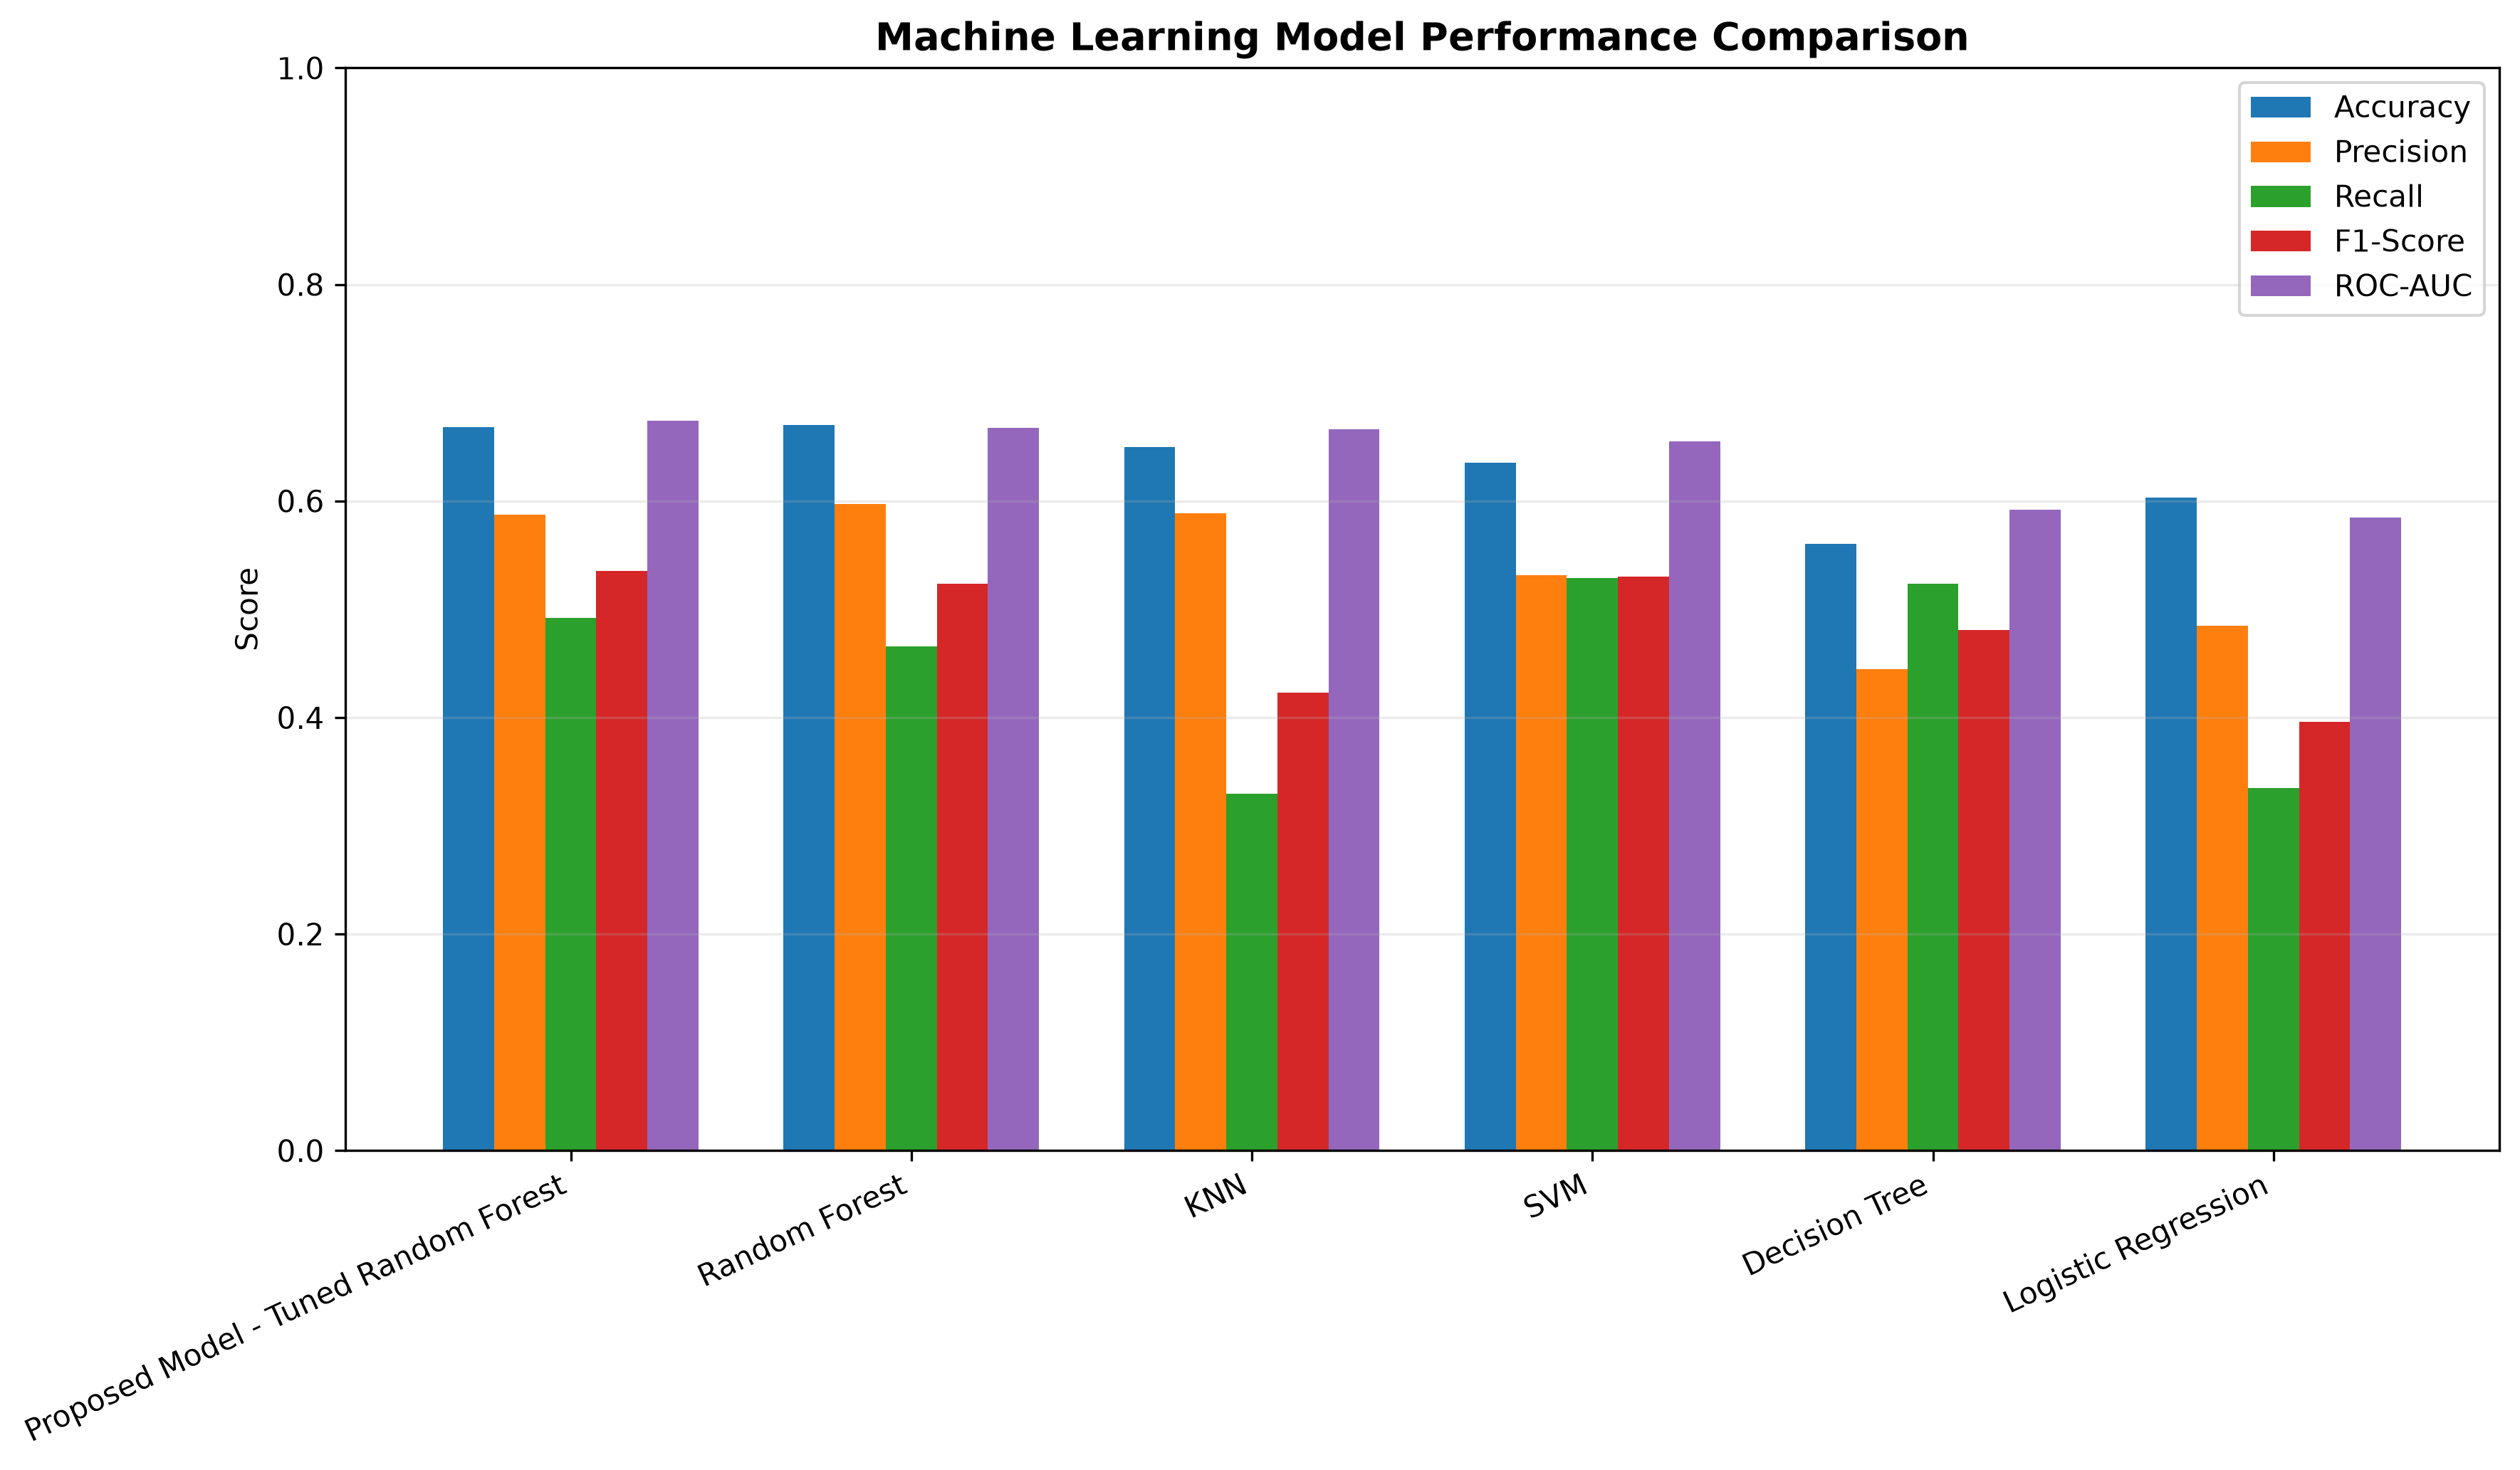
\includegraphics[width=0.88\textwidth]{model_comparison.png}
\caption{Multi-metric performance comparison (Accuracy, Precision, Recall, F1-Score, and ROC-AUC) across the six benchmarked classification models on the validation cohort.}\label{fig:model_comp}
\end{figure}

\begin{table}[t]
\caption{Repeated Stratified $5 \times 3$ CV ($n = 2,293$) and Held-Out Test Split ($n = 492$) benchmark results on the drinking-water dataset.}\label{tab:benchmark}%
\tiny\setlength{\tabcolsep}{1pt}
\begin{tabular*}{\textwidth}{@{\extracolsep\fill}lcccccccc@{}}
\toprule
Model & CV AUC & CV Acc & Test Acc [95\% CI] & Unsafe Rec & False-Safe & Potable F1 & Test AUC & Brier \\
\midrule
\textbf{Proposed Tuned RF} & $0.6960 \pm 0.0218$ & $0.6588$ & $\mathbf{0.6667}$ [62.39, 70.69\%] & $0.7733$ & $0.2267$ & $\mathbf{0.5393}$ & $0.6808$ & $0.2167$ \\
Random Forest & $0.6912 \pm 0.0196$ & $0.6585$ & $0.6585$ [61.56, 69.91\%] & $0.7667$ & $0.2333$ & $0.5281$ & $\mathbf{0.6898}$ & $\mathbf{0.2137}$ \\
SVM (RBF) & $\mathbf{0.7058 \pm 0.0235}$ & $\mathbf{0.6633}$ & $0.6220$ [57.83, 66.37\%] & $0.6767$ & $0.3233$ & $0.5255$ & $0.6581$ & $0.2180$ \\
KNN ($k=9$) & $0.6530 \pm 0.0219$ & $0.6412$ & $0.6382$ [59.48, 67.94\%] & $\mathbf{0.8333}$ & $\mathbf{0.1667}$ & $0.4183$ & $0.6156$ & $0.2365$ \\
Logistic Regression & $0.6211 \pm 0.0137$ & $0.6225$ & $0.6321$ [58.86, 67.35\%] & $0.7700$ & $0.2300$ & $0.4692$ & $0.6318$ & $0.2376$ \\
Decision Tree & $0.6198 \pm 0.0258$ & $0.6028$ & $0.5894$ [54.54, 63.20\%] & $0.6100$ & $0.3900$ & $0.5144$ & $0.6041$ & $0.2680$ \\
\botrule
\end{tabular*}
\end{table}

\begin{table}[t]
\caption{Nadeau--Bengio corrected resampled $t$-tests on Repeated $5 \times 3$ CV ROC-AUC ($df = 14$).}\label{tab:nadeau_t}%
\tiny\setlength{\tabcolsep}{1pt}
\begin{tabular}{@{}lcccc@{}}
\toprule
Model Comparison & Mean AUC Diff & $t_{\text{NB}}$ & $p$-value & Significant ($\alpha = 0.05$) \\
\midrule
SVM (RBF) vs. Proposed Tuned RF & $+0.0098$ & $+0.8617$ & $0.4034$ & False \\
Random Forest vs. Proposed Tuned RF & $-0.0047$ & $-1.2003$ & $0.2499$ & False \\
KNN ($k=9$) vs. Proposed Tuned RF & $-0.0430$ & $-3.8141$ & $0.0019$ & True \\
Logistic Regression vs. Proposed Tuned RF & $-0.0748$ & $-6.8511$ & $<0.0001$ & True \\
Decision Tree vs. Proposed Tuned RF & $-0.0762$ & $-5.1762$ & $0.0001$ & True \\
\botrule
\end{tabular}
\end{table}

Pairwise hypothesis testing using the Nadeau--Bengio corrected resampled $t$-test (Table~\ref{tab:nadeau_t}) reveals that neither RBF SVM ($t_{\text{NB}} = 0.8617, p = 0.4034$) nor default Random Forest ($t_{\text{NB}} = -1.2003, p = 0.2499$) differs significantly from the Tuned Random Forest at $\alpha = 0.05$. In contrast, Tuned RF significantly outperforms instance-based KNN ($p = 0.0019$), linear Logistic Regression ($p < 0.0001$), and orthogonal Decision Trees ($p = 0.0001$). 

On the held-out test split ($n = 492$), default Random Forest achieves a marginally higher ROC-AUC ($0.6898$) than the Tuned RF ($0.6808$, Figure~\ref{fig:roc}), while Tuned RF achieves the highest test accuracy ($66.67\%$ [95\% CI: $62.39\%, 70.69\%$]) and Potable F1 ($0.5393$). Figure~\ref{fig:confusion_matrix} displays the corresponding test confusion matrix at the default $0.50$ score cutoff.

\begin{figure}[h]
\centering
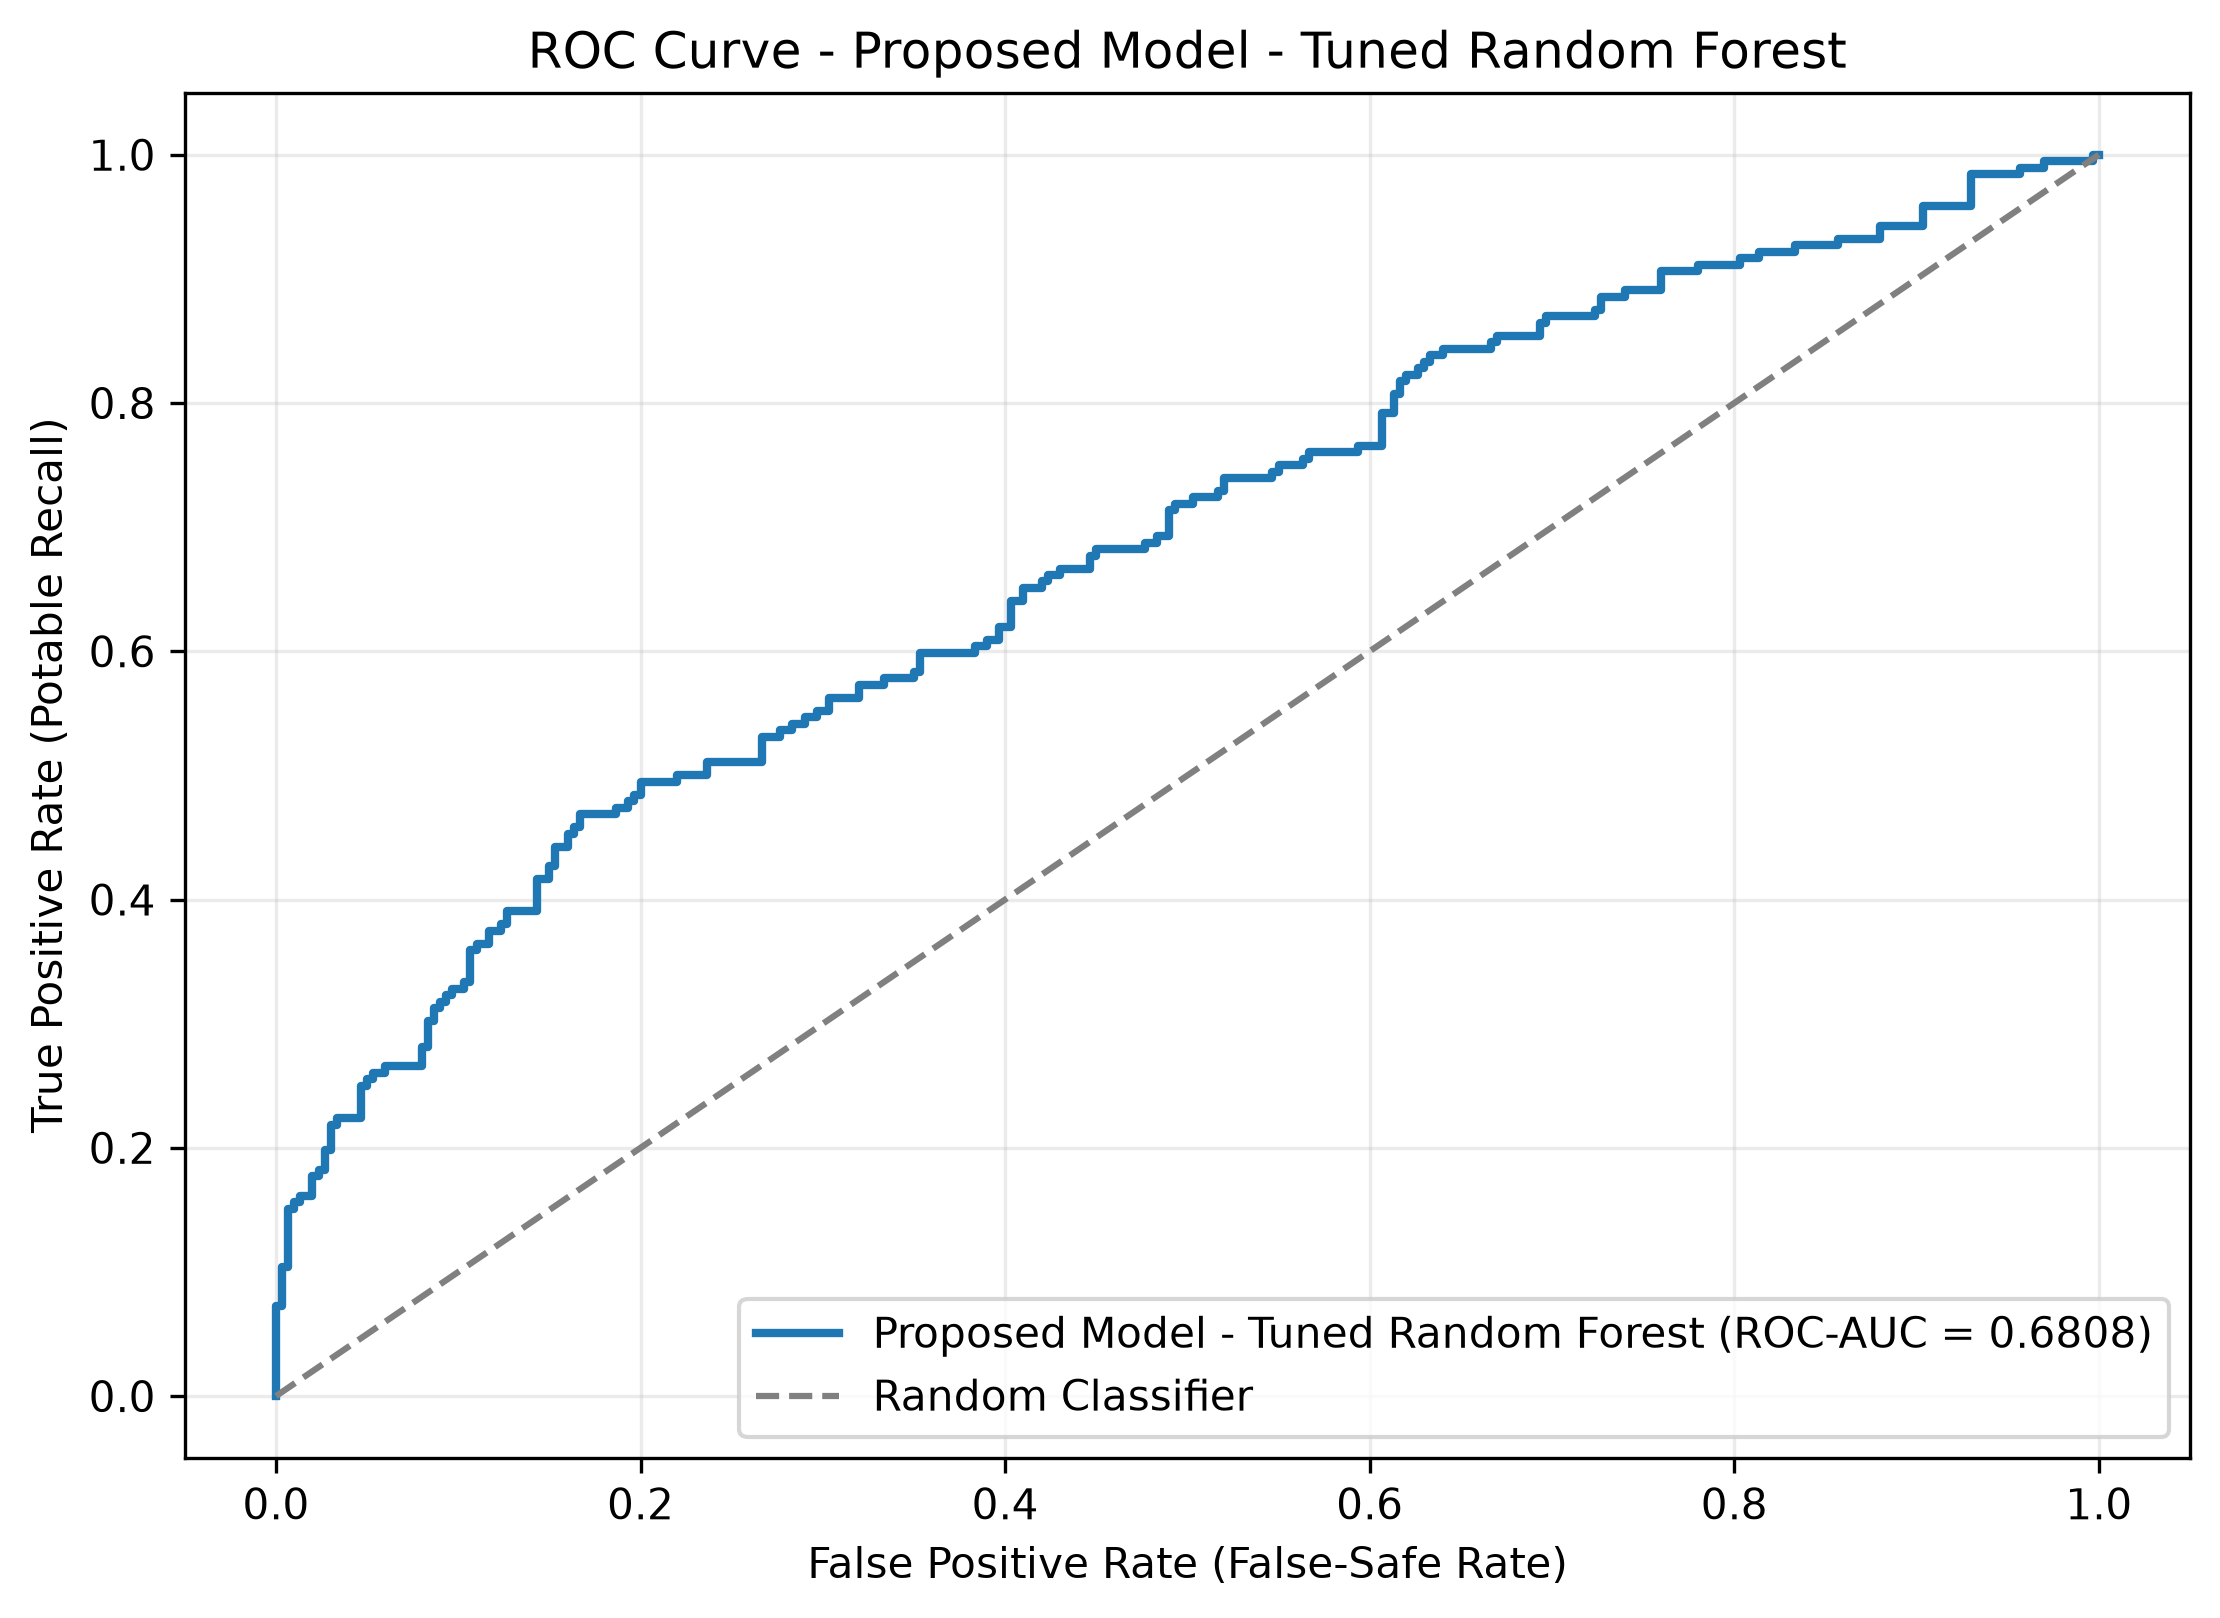
\includegraphics[width=0.70\textwidth]{roc_curve.png}
\caption{Receiver Operating Characteristic (ROC) curve of the Proposed Tuned Random Forest on the held-out test split ($n = 492$, $\text{ROC-AUC} = 0.6808$).}\label{fig:roc}
\end{figure}

\begin{figure}[h]
\centering
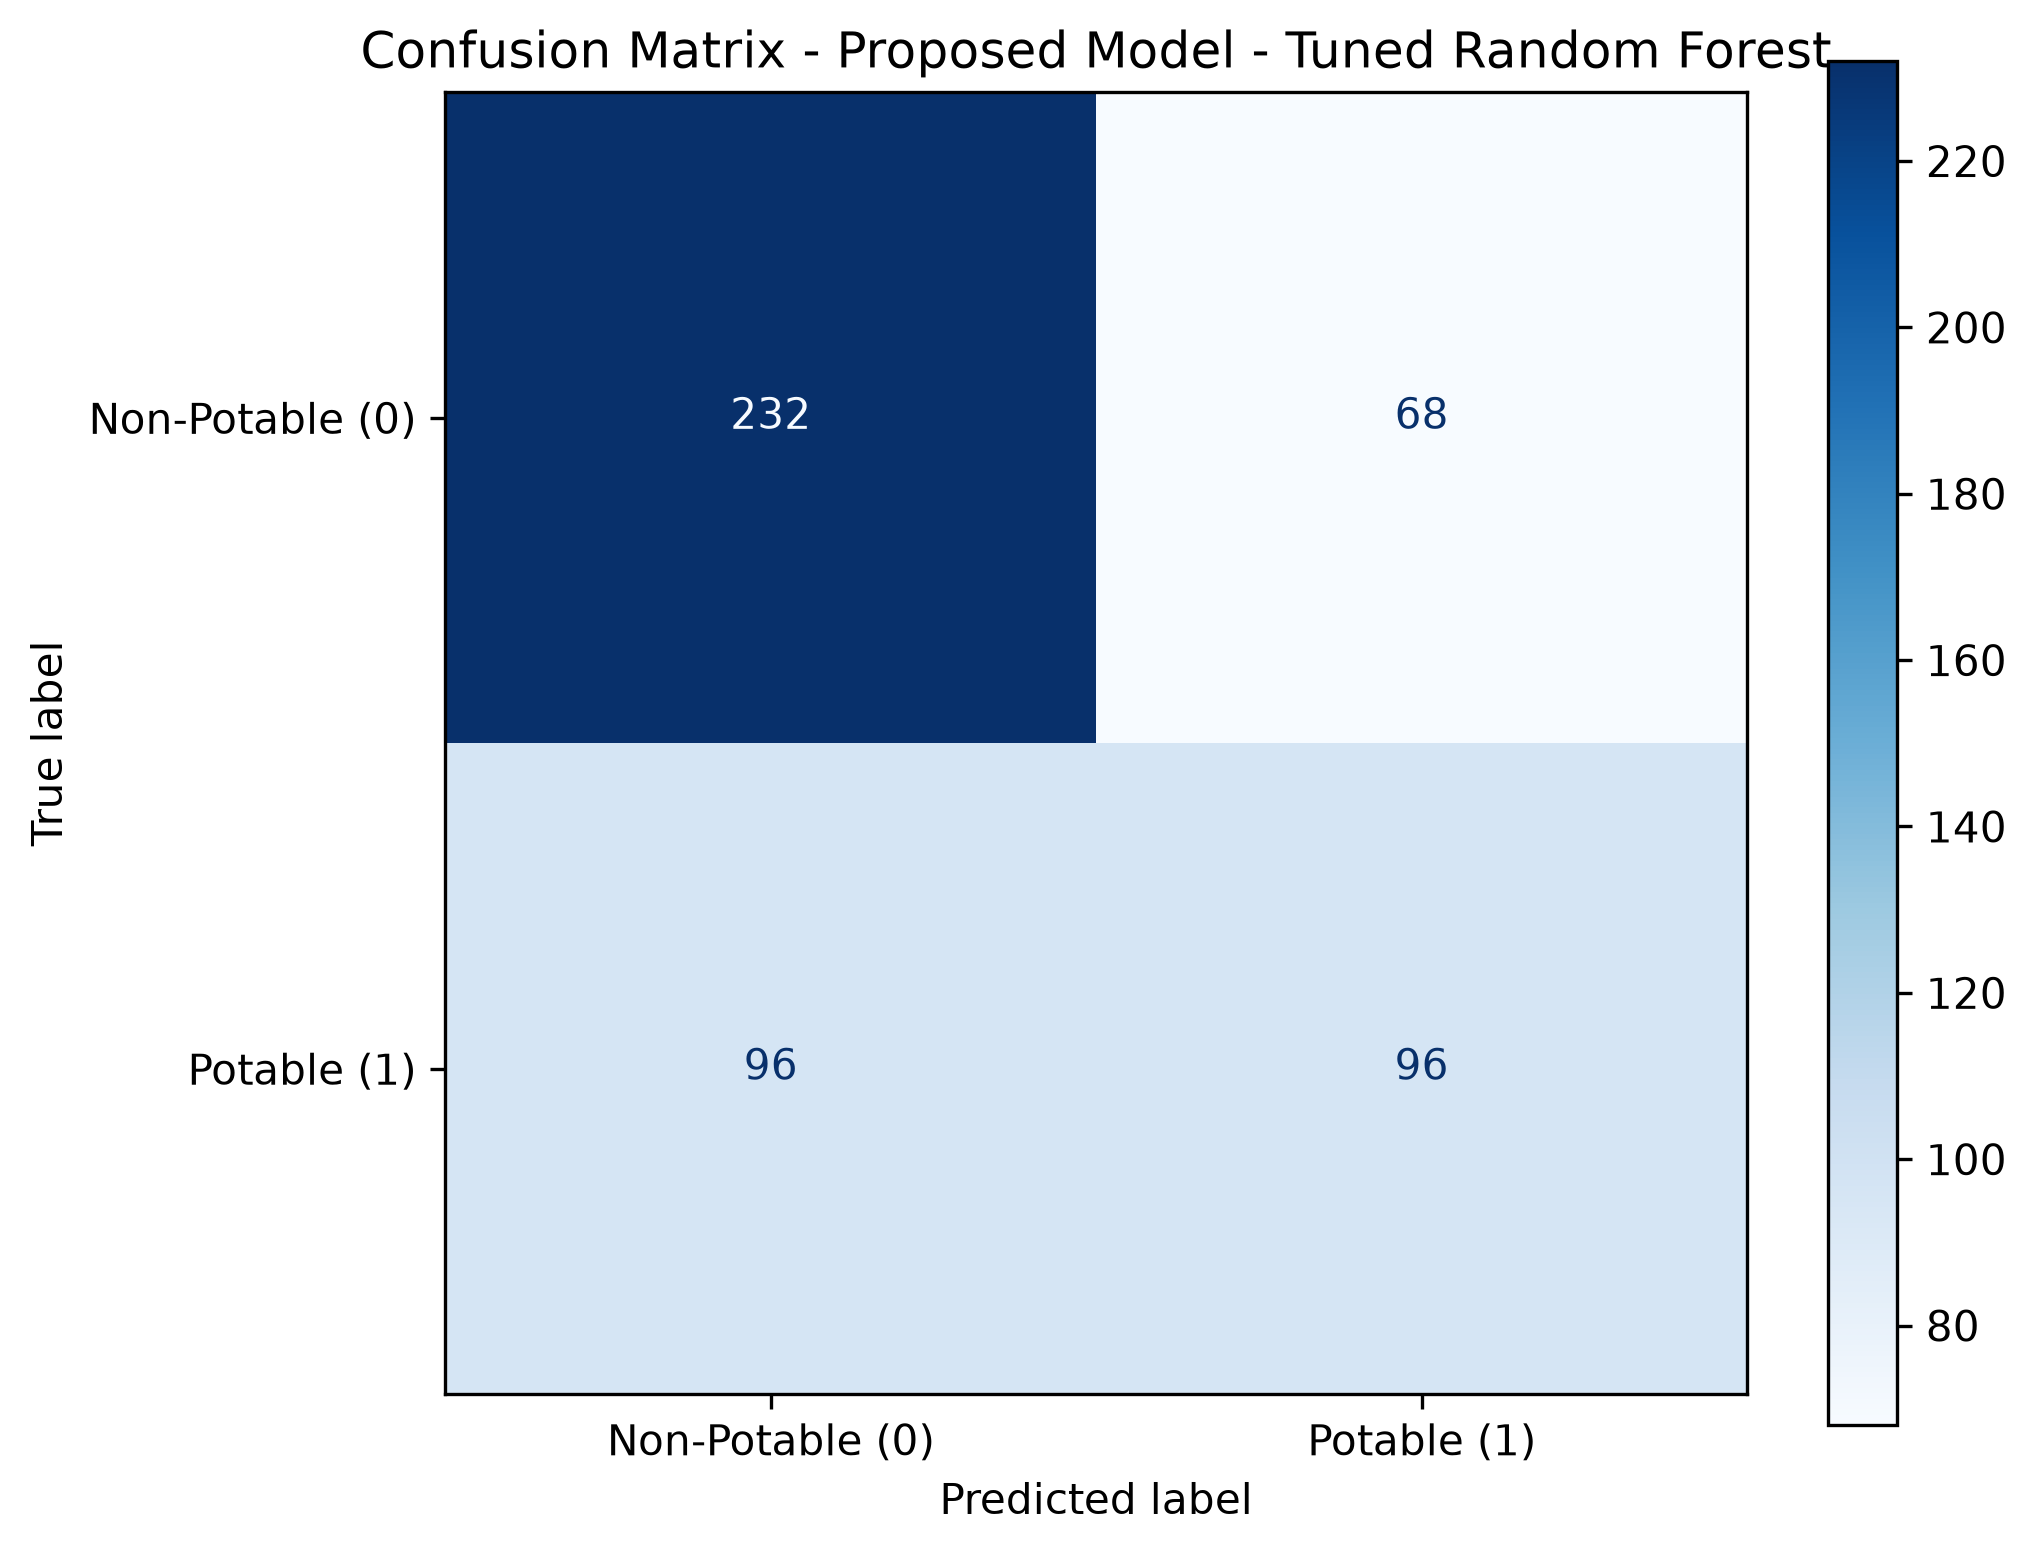
\includegraphics[width=0.66\textwidth]{confusion_matrix.png}
\caption{Confusion matrix of the Proposed Tuned Random Forest at the default $0.50$ score cutoff on the held-out test split ($n = 492$: $\text{TN}=232, \text{FP}=68, \text{FN}=96, \text{TP}=96$).}\label{fig:confusion_matrix}
\end{figure}

These findings yield an essential methodological conclusion: \textbf{extensive hyperparameter tuning provided no measurable generalization advantage over an untuned Random Forest}. Furthermore, compared with prior literature (e.g., Rachid et al. \cite{rachid2025}, where complete-case dropping and downsampling to $1,622$ samples caused SVM to degrade to $48\%$ accuracy and $0.47$ AUC while RF reported $0.75$ AUC), evaluating all $3,276$ records within an encapsulated, leak-free pipeline stabilizes RBF SVM ($0.7058$ CV AUC) and demonstrates that routine physicochemical indicators inherently plateau between $0.68$ and $0.71$ ROC-AUC.

\subsection{Experiment 2: Ablation Studies and Target-Leakage Audit}\label{subsec5_4}

To avoid using the held-out test split for exploratory architectural choices, all ablation experiments were conducted strictly across 5-fold Stratified CV on $\mathcal{D}_{\text{train}}$ ($n = 2,293$) and the validation partition $\mathcal{D}_{\text{val}}$ ($n = 491$), complemented by an empirical leakage audit:

\begin{enumerate}
\item \textit{Missing-Data Imputation Ablation (Table~\ref{tab:imputation}):} Comparing five imputation strategies inside the encapsulated pipeline indicates that multivariate ExtraTrees MICE \cite{vanbuuren2011} ($0.6964 \pm 0.0210$ CV AUC) and simple Median imputation ($0.6984 \pm 0.0152$ CV AUC) are statistically indistinguishable (paired $t = -0.5074, p = 0.6386$; validation exact binomial McNemar test \cite{mcnemar1947}: $b = 20, c = 19, p = 1.0000$). Furthermore, BayesianRidge MICE ($81.33\%$) and Median imputation ($80.67\%$) yield higher validation Unsafe Recall than ExtraTrees MICE ($78.00\%$). On weak-signal physicochemical tabular data, simple univariate median replacement matches multivariate iterative chaining while requiring orders of magnitude less computation.

\begin{table}[t]
\caption{Imputation strategy ablation on 5-fold Stratified CV ($\mathcal{D}_{\text{train}}$, $n = 2,293$) and Validation ($\mathcal{D}_{\text{val}}$, $n = 491$).}\label{tab:imputation}%
\tiny\setlength{\tabcolsep}{1pt}
\begin{tabular*}{\textwidth}{@{\extracolsep\fill}lcccccc@{}}
\toprule
Imputation Strategy & 5-Fold CV AUC & Val Acc & Val Unsafe Rec & Val False-Safe & Val Potable F1 & Val AUC \\
\midrule
1. Mean Imputation & $0.6971 \pm 0.0182$ & $0.6619$ & $0.8000$ & $0.2000$ & $0.5060$ & $0.6721$ \\
2. Median Imputation & $\mathbf{0.6984 \pm 0.0152}$ & $0.6660$ & $0.8067$ & $0.1933$ & $0.5090$ & $0.6682$ \\
3. KNN Imputation ($k=5$) & $0.6899 \pm 0.0145$ & $0.6517$ & $0.7700$ & $0.2300$ & $0.5100$ & $0.6691$ \\
4. MICE (BayesianRidge) & $0.6927 \pm 0.0160$ & $\mathbf{0.6741}$ & $\mathbf{0.8133}$ & $\mathbf{0.1867}$ & $0.5210$ & $0.6697$ \\
5. MICE (ExtraTrees) & $0.6964 \pm 0.0210$ & $0.6680$ & $0.7800$ & $0.2200$ & $\mathbf{0.5356}$ & $\mathbf{0.6728}$ \\
\botrule
\end{tabular*}
\end{table}

\item \textit{Ensemble and Class-Weighting Ablation (Table~\ref{tab:ensembles}):} Removing inverse-prevalence class weighting (\texttt{Unweighted Tuned RF}) elevates validation Unsafe Recall from $78.00\%$ to $94.00\%$ (reducing the False-Safe Rate from $22.00\%$ to $6.00\%$), because the unweighted model defaults toward the non-potable majority class ($60.99\%$), sacrificing Potable Recall ($26.18\%$). Blending models via Soft-Voting \cite{dietterich2000} ($0.6714$ Val AUC) or Stacking \cite{wolpert1992} ($0.6703$ Val AUC) fails to improve validation ROC-AUC over a single Tuned RF ($0.6739$).

\begin{table}[t]
\caption{Ensemble and class-weighting ablation on 5-fold CV ($\mathcal{D}_{\text{train}}$) and Validation ($\mathcal{D}_{\text{val}}$, $n = 491$).}\label{tab:ensembles}%
\tiny\setlength{\tabcolsep}{1pt}
\begin{tabular*}{\textwidth}{@{\extracolsep\fill}lccccccc@{}}
\toprule
Architecture & CV AUC & Val Acc & Val Unsafe Rec & Val False-Safe & Val Potable Rec & Val F1 & Val AUC \\
\midrule
Tuned RF (Balanced) & $0.6981$ & $0.6680$ & $0.7800$ & $0.2200$ & $0.4921$ & $\mathbf{0.5356}$ & $\mathbf{0.6739}$ \\
Unweighted Tuned RF & $0.6935$ & $\mathbf{0.6762}$ & $\mathbf{0.9400}$ & $\mathbf{0.0600}$ & $0.2618$ & $0.3861$ & $0.6604$ \\
Extra Trees (Balanced) \cite{geurts2006} & $0.7026$ & $0.6701$ & $0.8367$ & $0.1633$ & $0.4084$ & $0.4906$ & $0.6652$ \\
Soft-Voting (RF+ET+SVM) & $0.7132$ & $\mathbf{0.6762}$ & $0.8567$ & $0.1433$ & $0.3927$ & $0.4854$ & $0.6714$ \\
Stacking (Meta-LR) & $\mathbf{0.7134}$ & $0.6253$ & $0.6833$ & $0.3167$ & $\mathbf{0.5340}$ & $0.5258$ & $0.6703$ \\
\botrule
\end{tabular*}
\end{table}

\item \textit{Empirical Target-Leakage Audit:} To empirically uncover why published studies report $>80\%$ accuracy on this benchmark, we reproduced class-conditional mean imputation applied prior to train--test partitioning (\texttt{df.groupby('Potability').transform('mean')}). Evaluated on the canonical $85/15$ split (\texttt{random\_state=42}), the target-leaky pipeline achieved $\mathbf{79.47\%}$ \textbf{test accuracy} ($\text{F1} = 0.7021$, $\mathbf{0.8798}$ \textbf{ROC-AUC}), whereas an encapsulated \texttt{SimpleImputer(strategy='mean')} fitted strictly on training data yielded $\mathbf{68.29\%}$ \textbf{accuracy} ($\text{F1} = 0.4507$, $\mathbf{0.6735}$ \textbf{ROC-AUC}), an inflation of $+11.18\%$ accuracy and $+0.2063$ ROC-AUC. Repeating this audit across $20$ stratified $85/15$ random seeds confirmed the systematic nature of this artifact: the leaky pipeline averaged $\mathbf{80.01 \pm 1.75\%}$ accuracy ($0.8779 \pm 0.0183$ ROC-AUC; $\text{F1} = 0.7144 \pm 0.0276$) compared with $\mathbf{67.12 \pm 1.71\%}$ accuracy ($0.6877 \pm 0.0277$ ROC-AUC; $\text{F1} = 0.4492 \pm 0.0390$) for the leak-free pipeline, yielding a mean inflation of $\mathbf{+12.89 \pm 1.54}$ \textbf{percentage points} in accuracy and $\mathbf{+0.1902 \pm 0.0210}$ in ROC-AUC \cite{kapoor2023,kaufman2012}.
\end{enumerate}

\subsection{Experiment 3: Risk-Sensitive Decision Thresholding and Probability Calibration}\label{subsec5_5}

In public-health screening, classification errors exhibit severe cost asymmetry: $\mathcal{C}(\text{False Safe}) \gg \mathcal{C}(\text{False Alarm})$. Mislabeling toxic water as potable directly exposes human populations to waterborne morbidity, whereas mislabeling safe water as non-potable incurs secondary laboratory confirmatory assays. 

\begin{table}[t]
\caption{Frozen operating-point comparison and probability calibration on the held-out test split ($n = 492$).}\label{tab:threshold_calib}%
\tiny\setlength{\tabcolsep}{1pt}
\begin{tabular*}{\textwidth}{@{\extracolsep\fill}lcccccc@{}}
\toprule
Operating Point / Calibration & Test Acc & Unsafe Rec & False-Safe & Potable Rec & Safe Rejected & Brier (BSS) \\
\midrule
Always-Predict-Prevalence Baseline & --- & --- & --- & --- & --- & $0.2380$ ($0.0000$) \\
Default Score Cutoff ($0.50$, Raw RF) & $0.6667$ & $0.7733$ & $0.2267$ & $\mathbf{0.5000}$ & $\mathbf{50.00\%}$ & $0.2167$ ($0.0891$) \\
Frozen Safety-First Cutoff ($0.60$, Val) & $\mathbf{0.6789}$ & $\mathbf{0.9500}$ & $\mathbf{0.0500}$ & $0.2552$ & $74.48\%$ & --- \\
Isotonic-Calibrated RF (Fit on Val) & --- & --- & --- & --- & --- & $\mathbf{0.2090}$ ($\mathbf{0.1219}$) \\
\botrule
\end{tabular*}
\end{table}

Sweeping decision thresholds over $\tau \in [0.30, 0.70]$ on $\mathcal{D}_{\text{val}}$ established $\tau^* = 0.60$ as an optimal safety-first cutoff ($95.67\%$ validation Unsafe Recall; $4.33\%$ False-Safe Rate). Freezing $\tau^* = 0.60$ on validation and applying it directly to $\mathcal{D}_{\text{test}}$ ($n = 492$, Table~\ref{tab:threshold_calib}) successfully depresses the test False-Safe Rate from $22.67\%$ to $\mathbf{5.00\%}$ ($95.00\%$ Unsafe Recall). However, this public-health protection incurs an operational cost: \textbf{the model rejects $\mathbf{74.48\%}$ of genuinely potable water} (Potable Recall drops from $50.00\%$ to $25.52\%$). This trade-off confirms that routine physicochemical sensors can serve for risk screening, but cannot replace microbiological certification.

\begin{figure}[h]
\centering
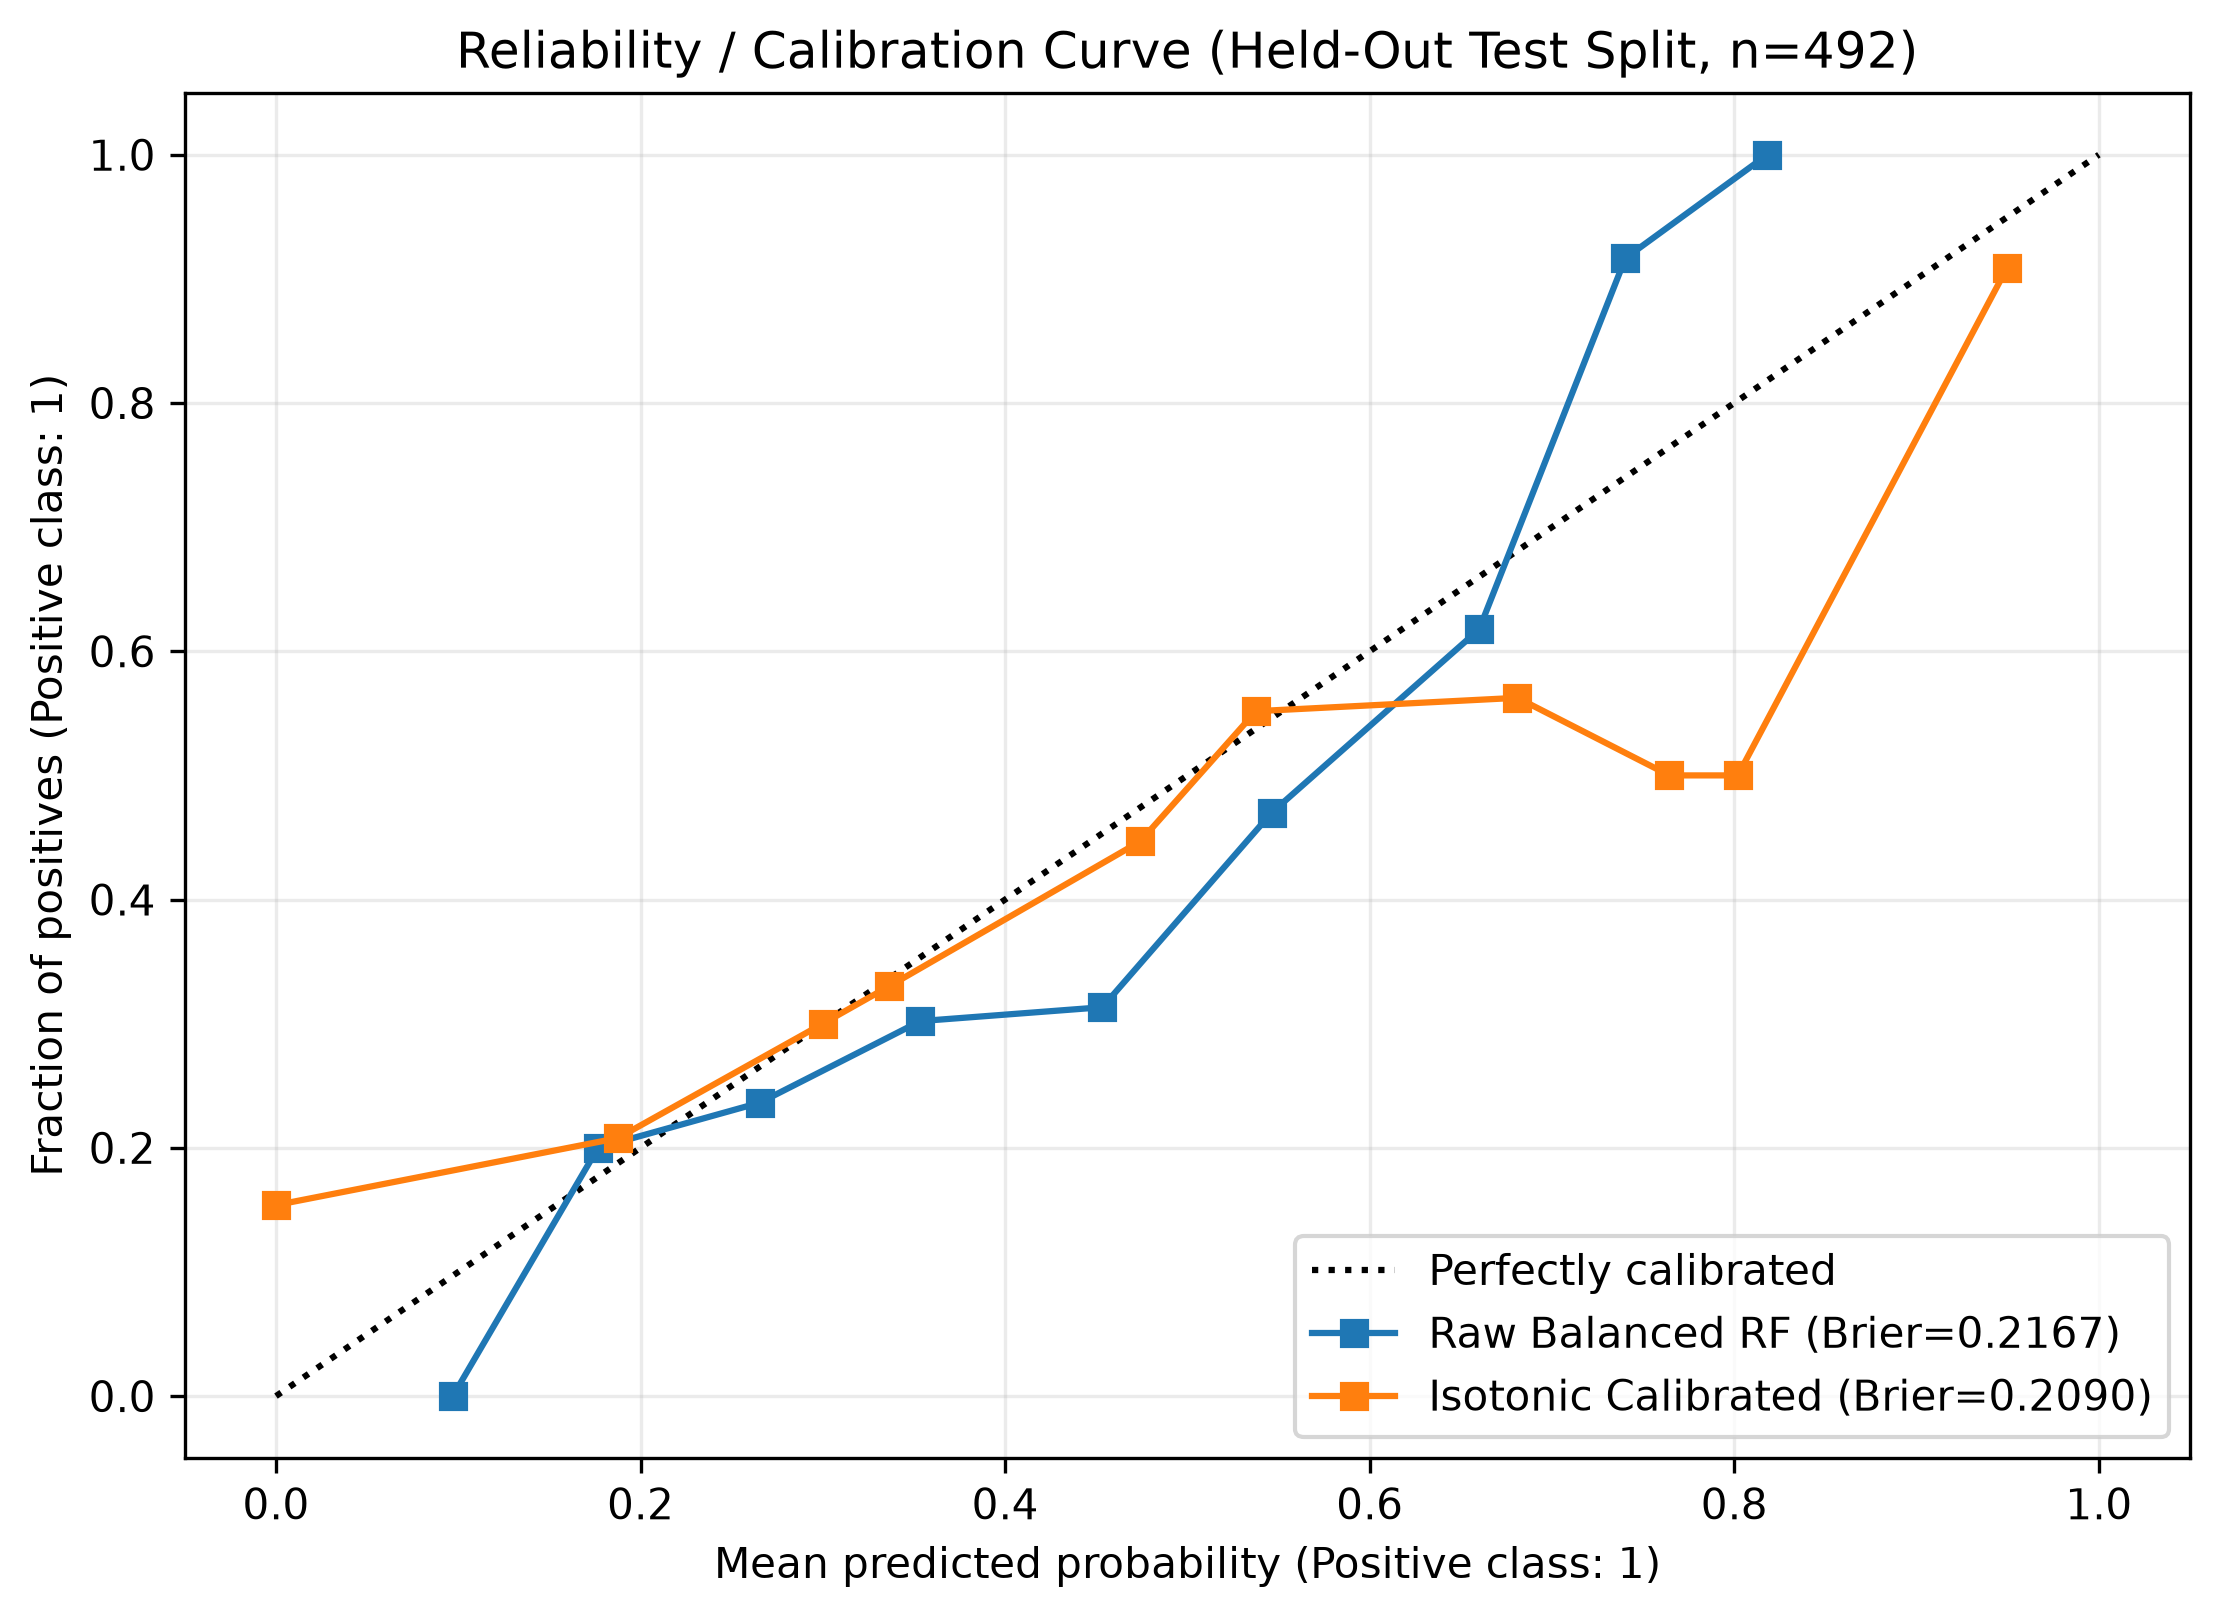
\includegraphics[width=0.70\textwidth]{calibration_curve.png}
\caption{Reliability (calibration) curves comparing uncalibrated balanced RF scores ($\text{Brier} = 0.2167$) against validation-fitted isotonic calibration ($\text{Brier} = 0.2090$) on the held-out test split ($n = 492$).}\label{fig:calibration}
\end{figure}

\begin{figure}[h]
\centering
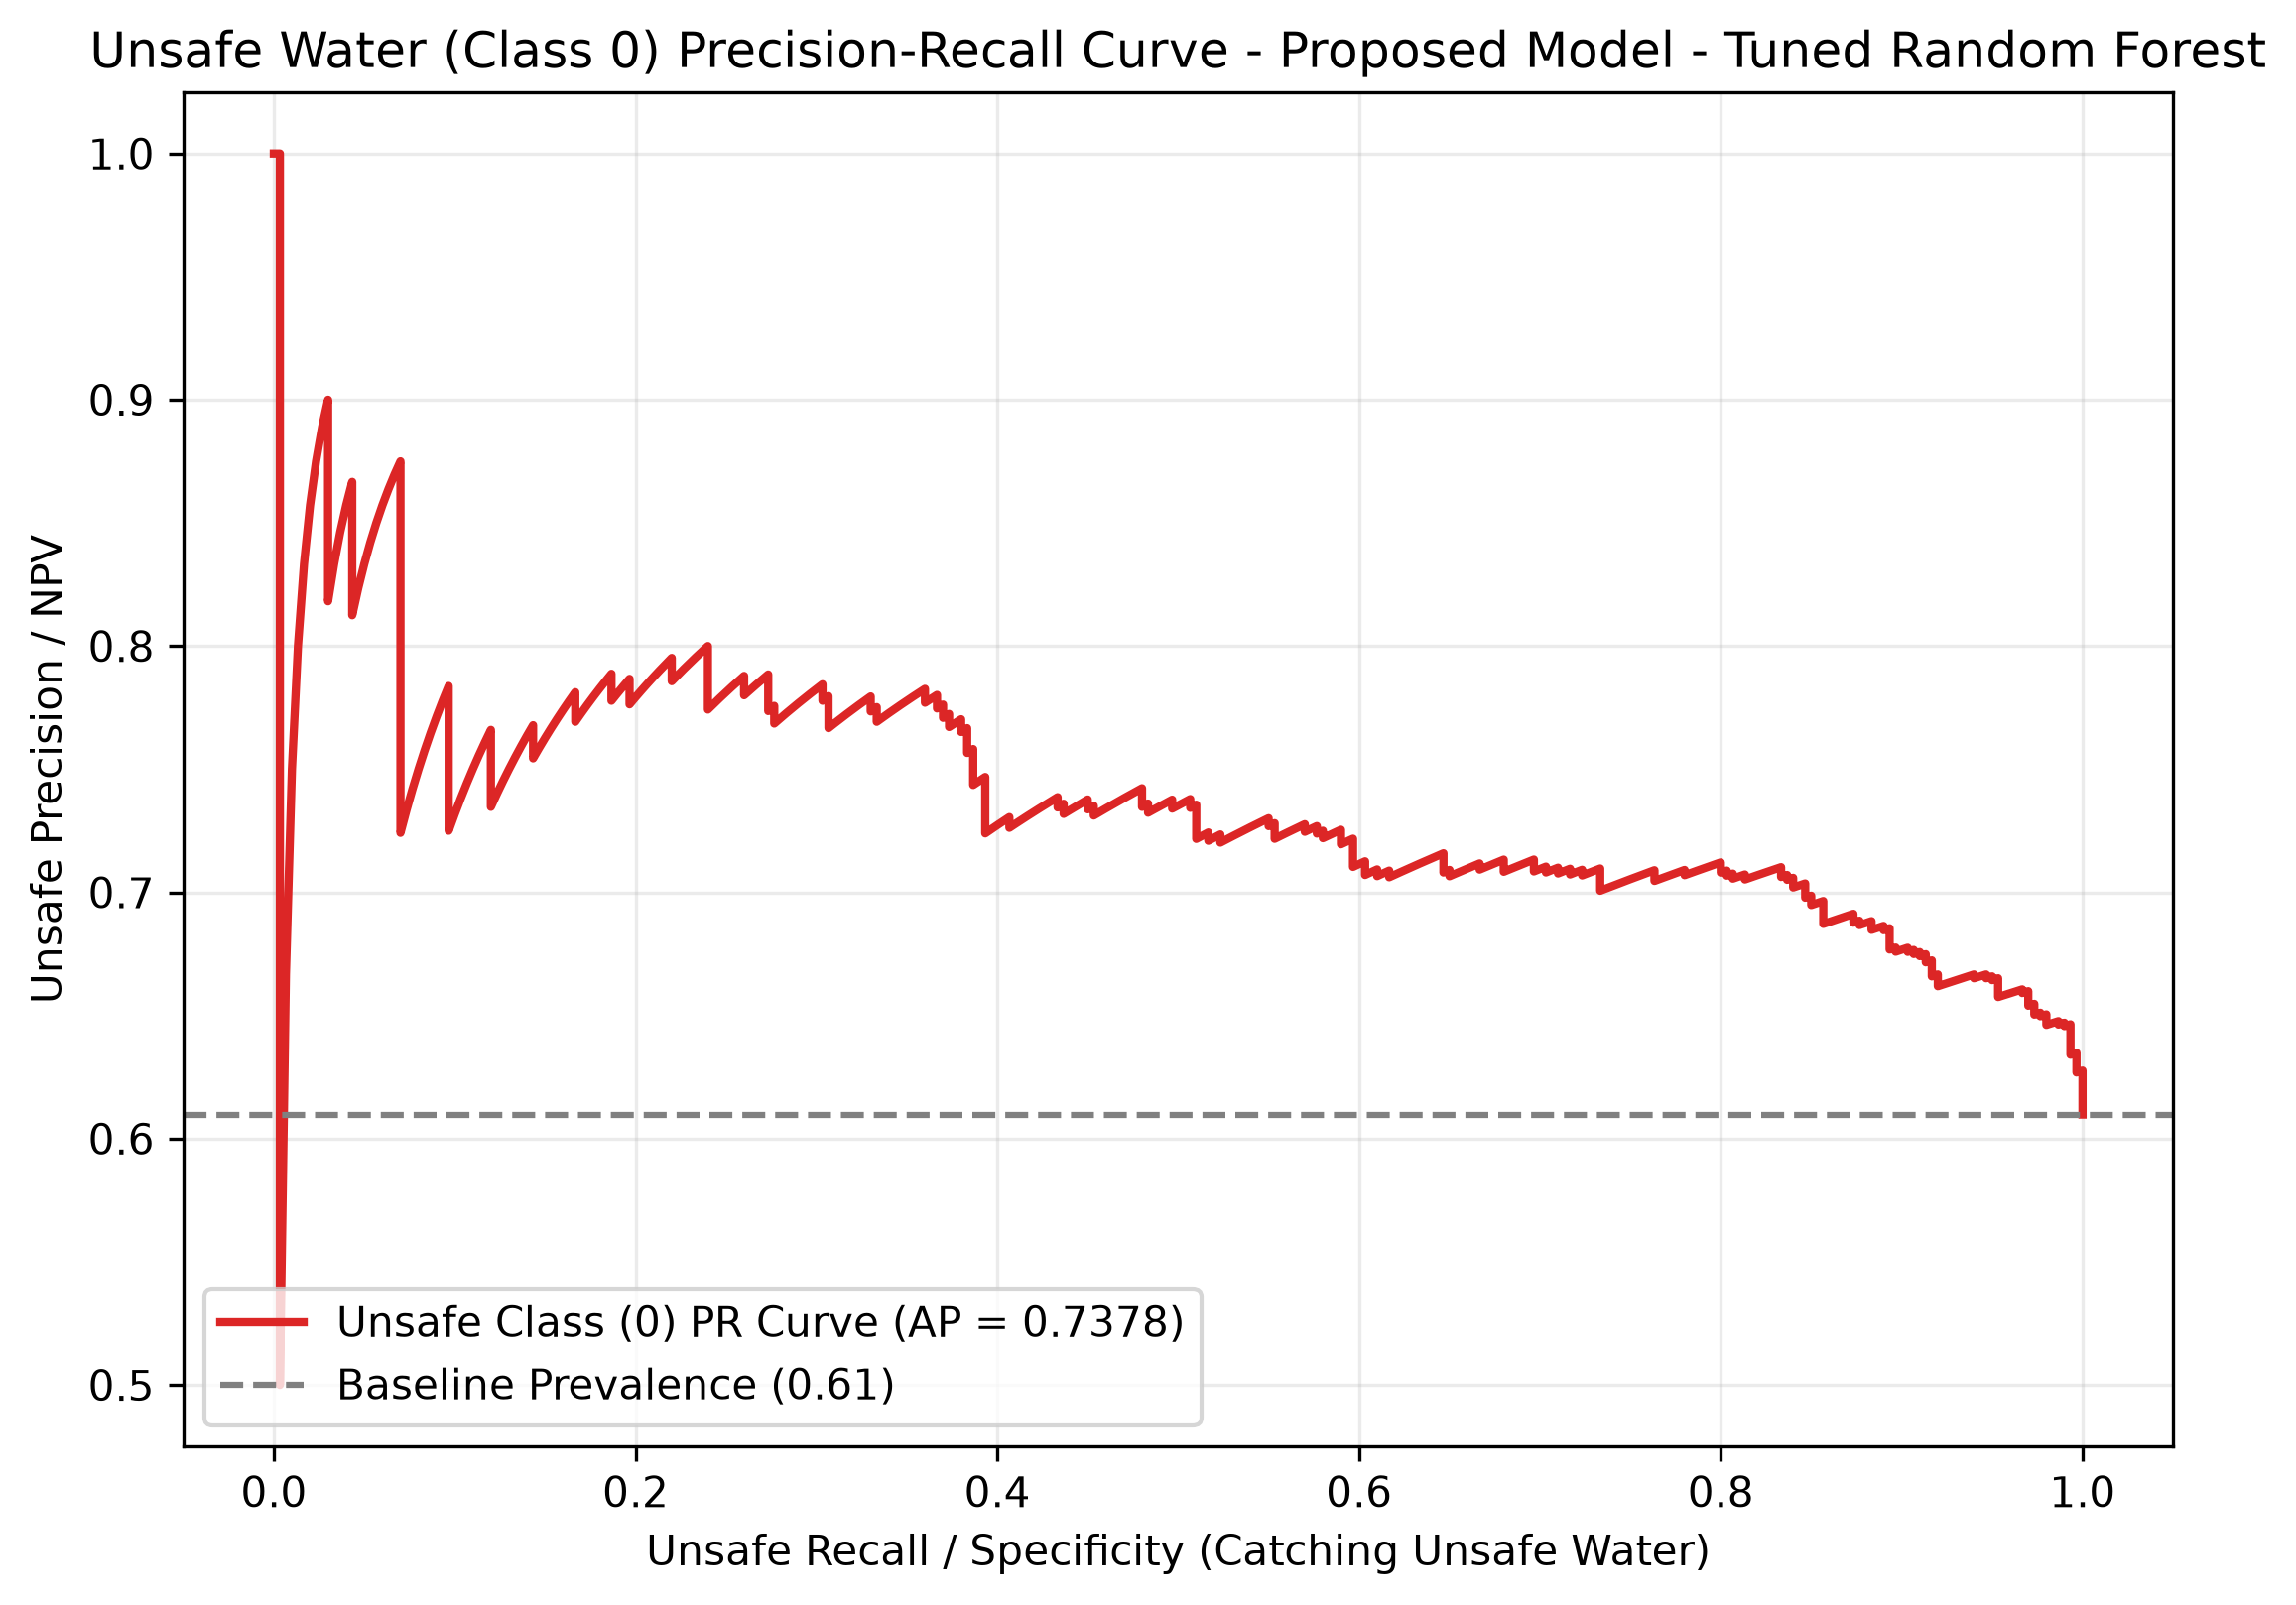
\includegraphics[width=0.70\textwidth]{unsafe_pr_curve.png}
\caption{Precision--Recall curve for Class-0 (Unsafe Water) on the held-out test split ($n = 492$), emphasizing high-recall operating regimes to suppress false-safe errors.}\label{fig:unsafe_pr}
\end{figure}

Because \texttt{class\_weight='balanced'} distorts ensemble vote fractions away from true event likelihoods, raw scores must be calibrated prior to risk communication. Fitting non-parametric \texttt{IsotonicRegression} \cite{niculescumizil2005} on $\mathcal{D}_{\text{val}}$ improves test Brier score from $0.2167$ ($\text{BSS} = 0.0891$) to $\mathbf{0.2090}$ ($\mathbf{BSS} = \mathbf{0.1219}$, Figure~\ref{fig:calibration}). The Class-0 (Unsafe Water) Precision--Recall curve is plotted in Figure~\ref{fig:unsafe_pr}.

\subsection{Experiment 4: Model Interpretability via TreeSHAP}\label{subsec5_6}

TreeSHAP attribution \cite{lundberg2017,lundberg2020} on the serialized production model (\texttt{best\_model\_pipeline.joblib}, Figure~\ref{fig:shap_summary}) ranks feature influence by mean absolute SHAP value: \texttt{ph} ($0.04226$), \texttt{Sulfate} ($0.04072$), \texttt{ph\_sulfate\_ratio} ($0.02993$), \texttt{Hardness} ($0.02433$), and \texttt{Chloramines} ($0.02026$). 

\begin{figure}[h]
\centering
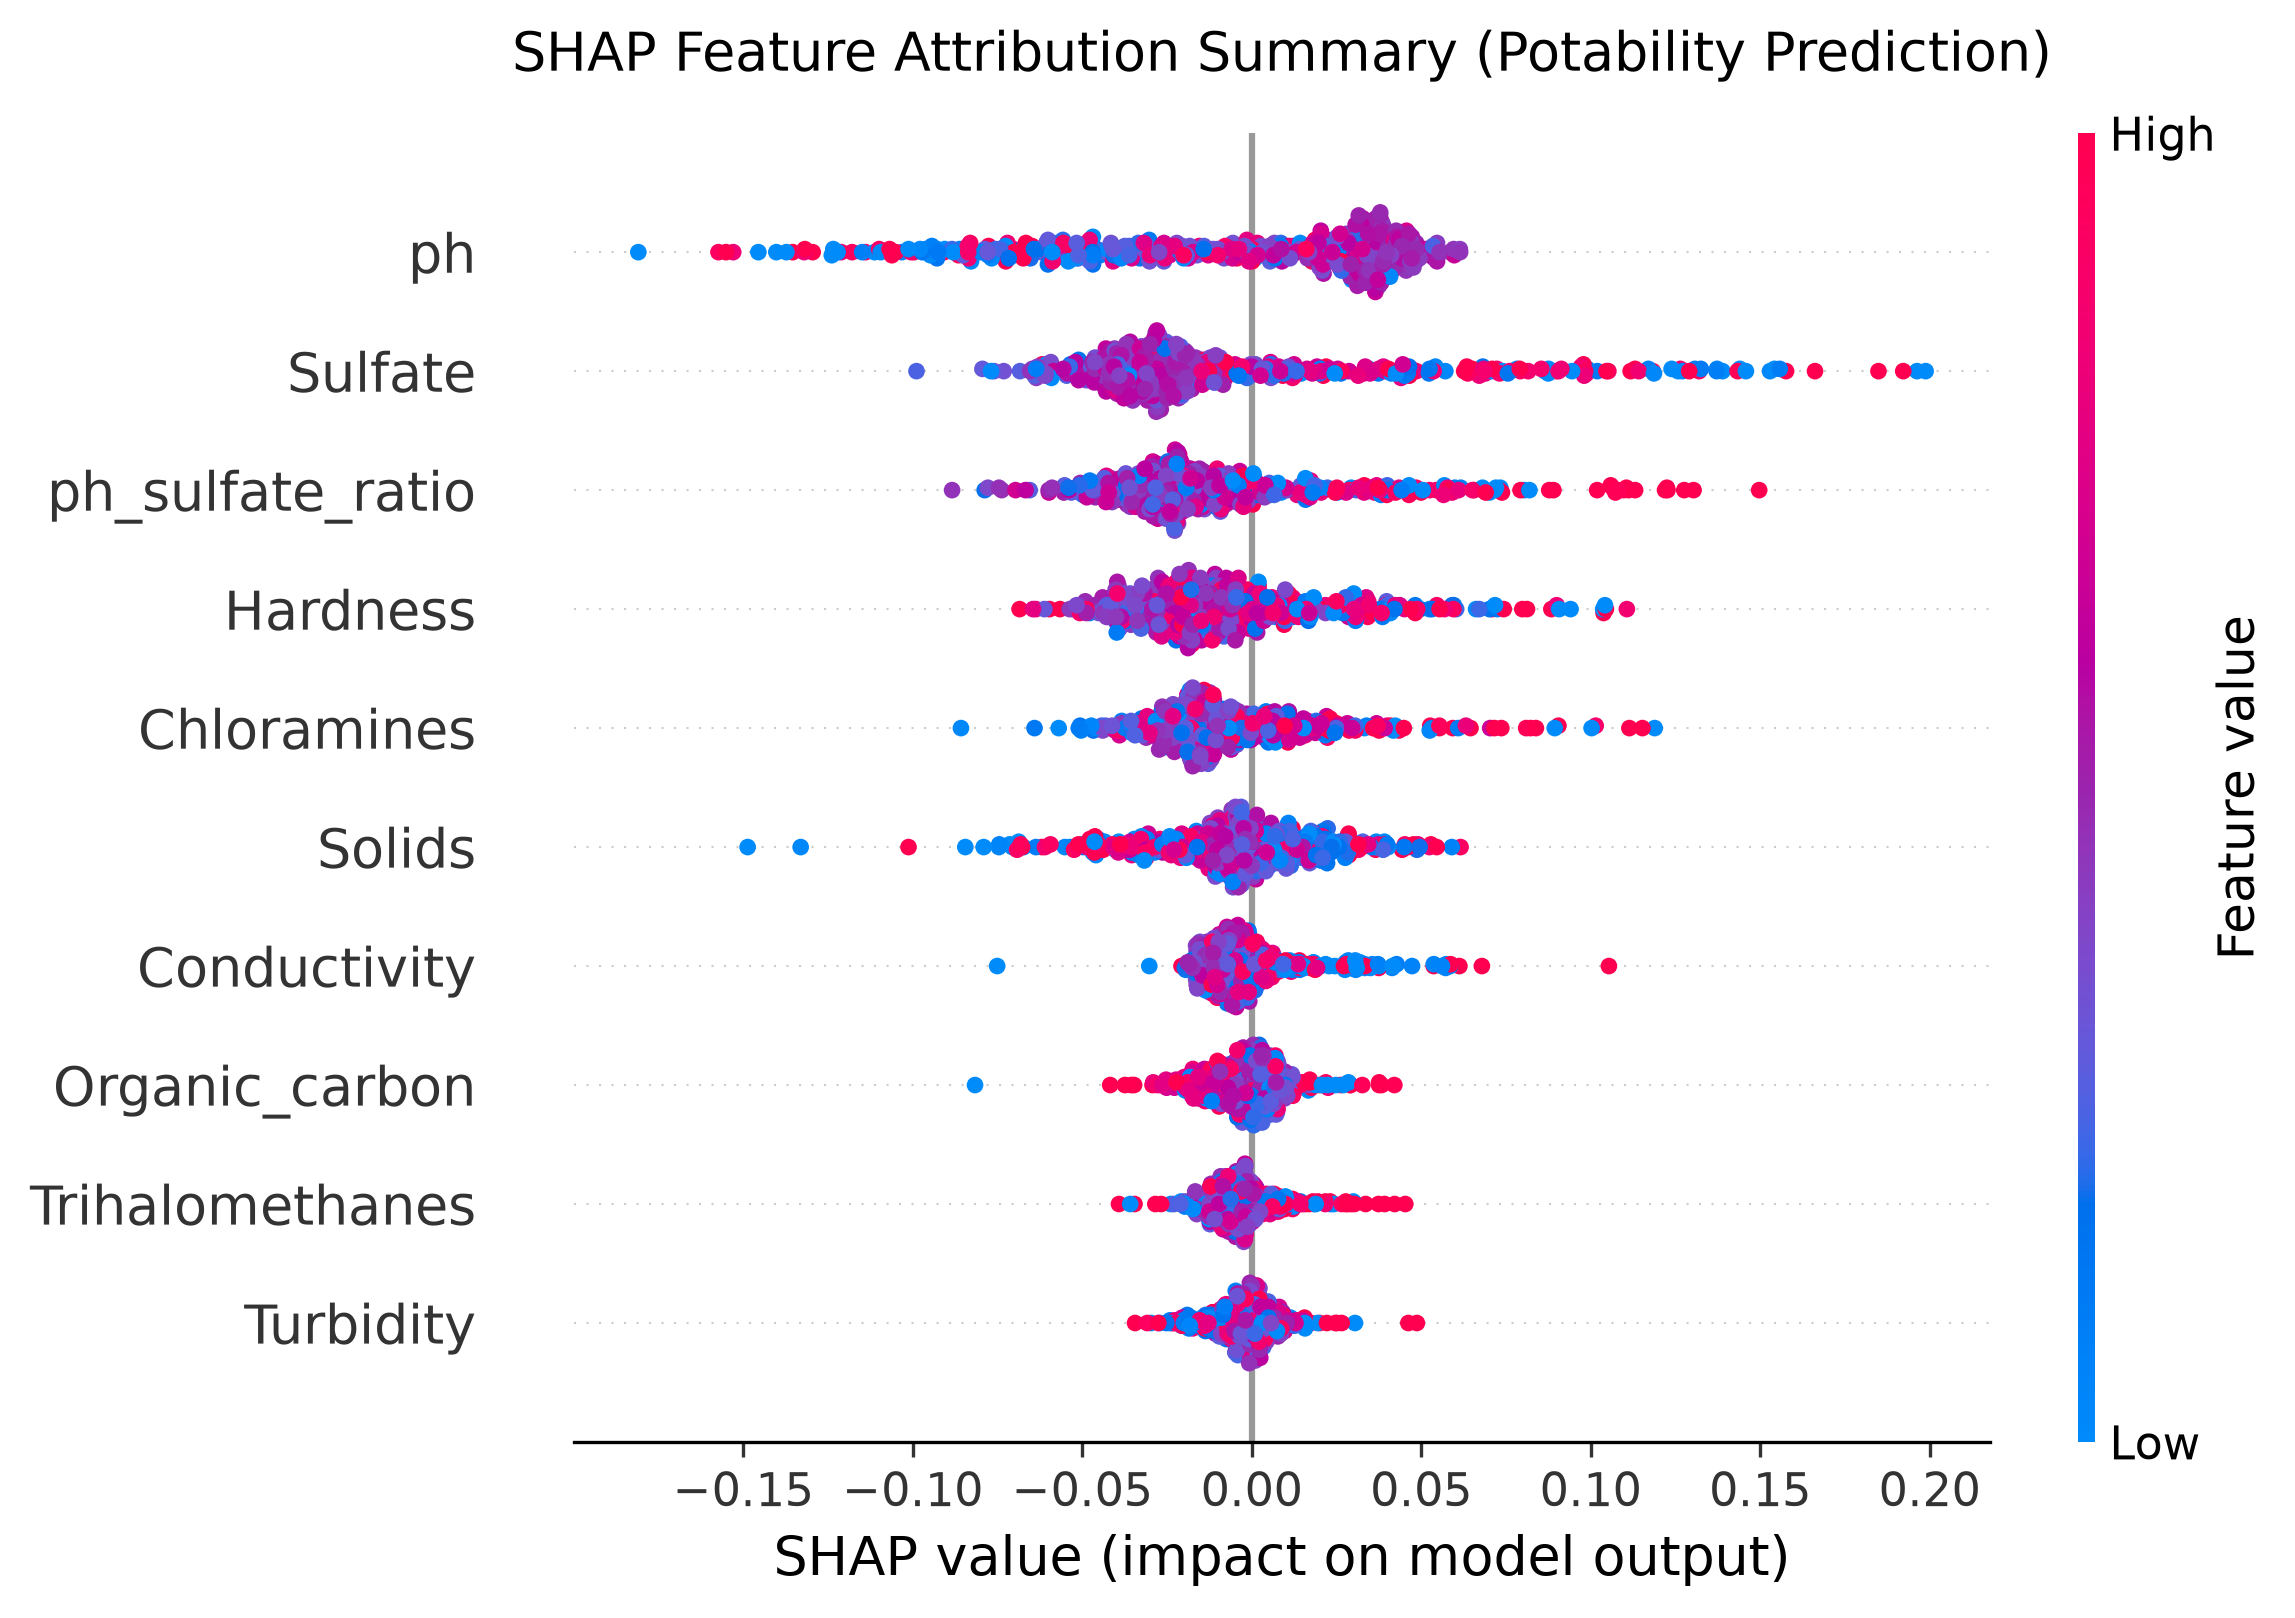
\includegraphics[width=0.76\textwidth]{shap_summary_plot.png}
\caption{TreeExplainer SHAP beeswarm summary plot on the held-out test split ($n = 492$) generated from \texttt{best\_model\_pipeline.joblib}.}\label{fig:shap_summary}
\end{figure}

The beeswarm distribution reveals that mid-range pH ($6.5$--$8.5$) yields positive SHAP values promoting potability, whereas extreme acidification ($\text{pH} < 6.5$) and alkalinization ($\text{pH} > 8.5$) strongly depress potability predictions. Figure~\ref{fig:shap_dependence} presents the SHAP partial dependence plot for the engineered acid--base mineralization index (\texttt{ph\_sulfate\_ratio}) conditioned on pH.

\begin{figure}[h]
\centering
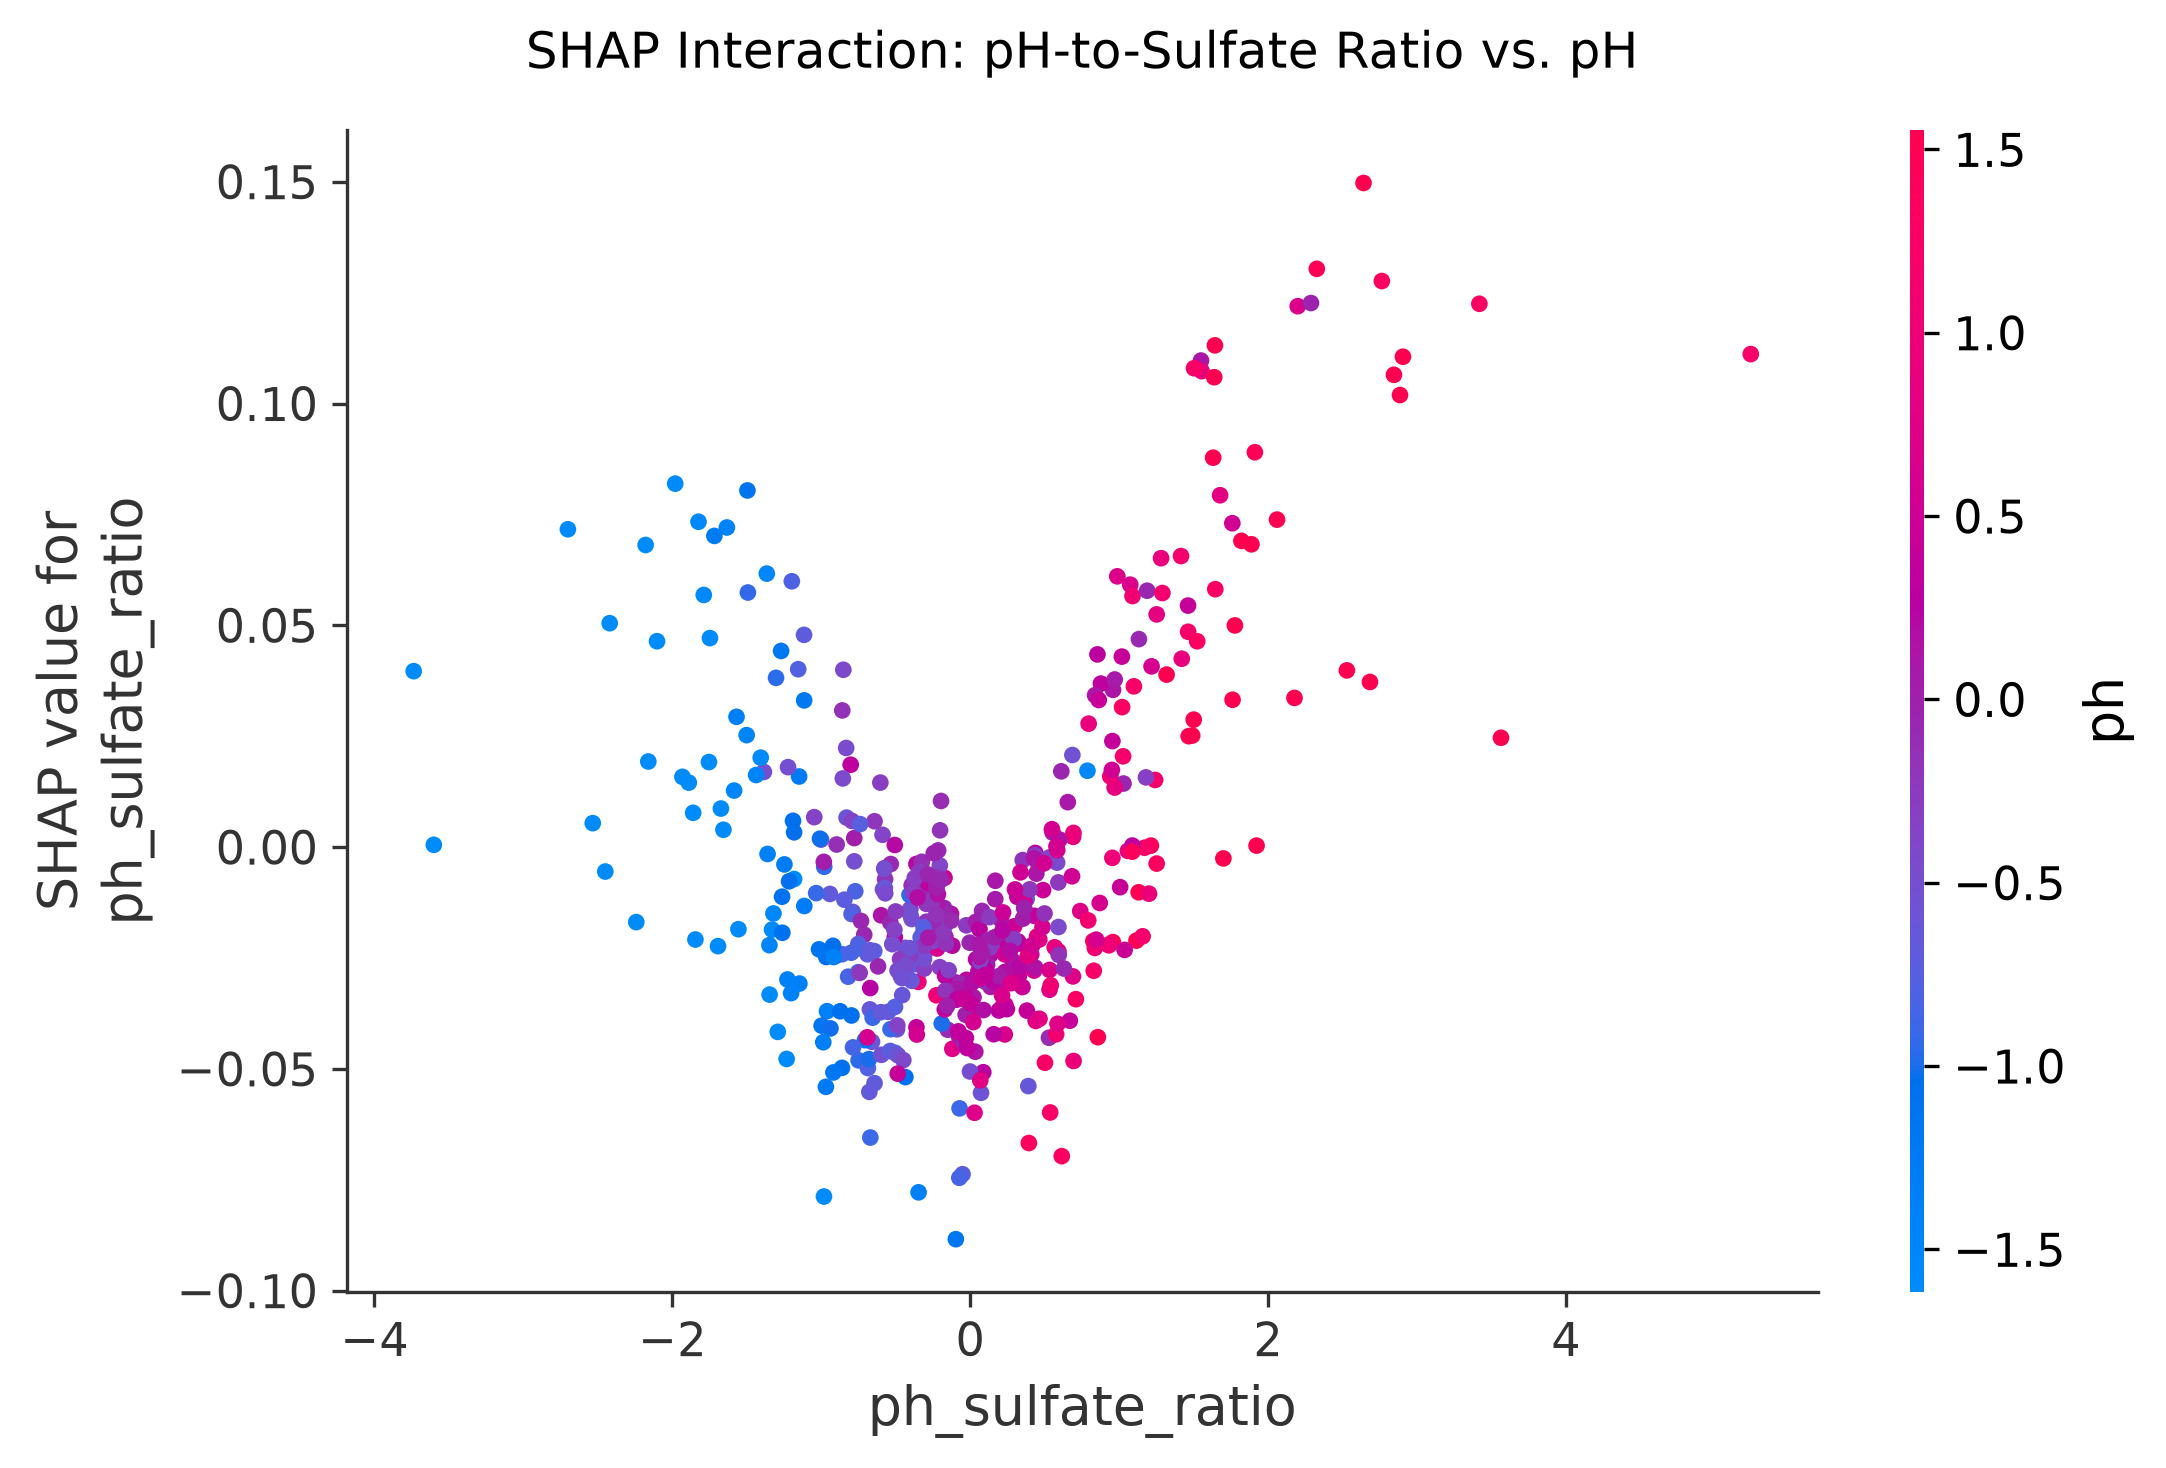
\includegraphics[width=0.72\textwidth]{shap_dependence_ratio.png}
\caption{TreeSHAP partial dependence and interaction plot for the engineered acid--base mineralization index (\texttt{ph\_sulfate\_ratio}) conditioned on pH, highlighting non-linear operational margins.}\label{fig:shap_dependence}
\end{figure}

Because $\text{ph\_sulfate\_ratio}$ is a deterministic mathematical transform of \texttt{ph} and \texttt{Sulfate}, TreeSHAP splits credit across the collinear features rather than identifying independent chemical mechanisms. This underscores the necessity of auditing engineered features for collinear credit splitting in explainable machine learning.

\subsection{Regional Surface-Water Case Study: Indian CPCB Spatial Generalization}\label{subsec5_7}

The regional case study evaluates $N = 683$ lentic monitoring stations across 26 Indian States/UTs \cite{cpcb2024}. Figure~\ref{fig:india_state_pollution} illustrates the spatial variation in water quality degradation across the 26 administrative divisions. Industrialized basins such as Karnataka ($79.26\%, n = 188$) and Telangana ($76.51\%, n = 149$) exhibit high contamination burdens, contrasted with pristine or protected regions such as Tripura ($0.00\%, n = 18$) and Andhra Pradesh ($5.26\%, n = 19$). Across freshwater body classifications, Tanks exhibit the highest degradation proportion ($54.08\%, n = 98$), followed by Lakes ($47.54\%, n = 488$) and Ponds ($29.90\%, n = 97$).

\begin{figure}[h]
\centering
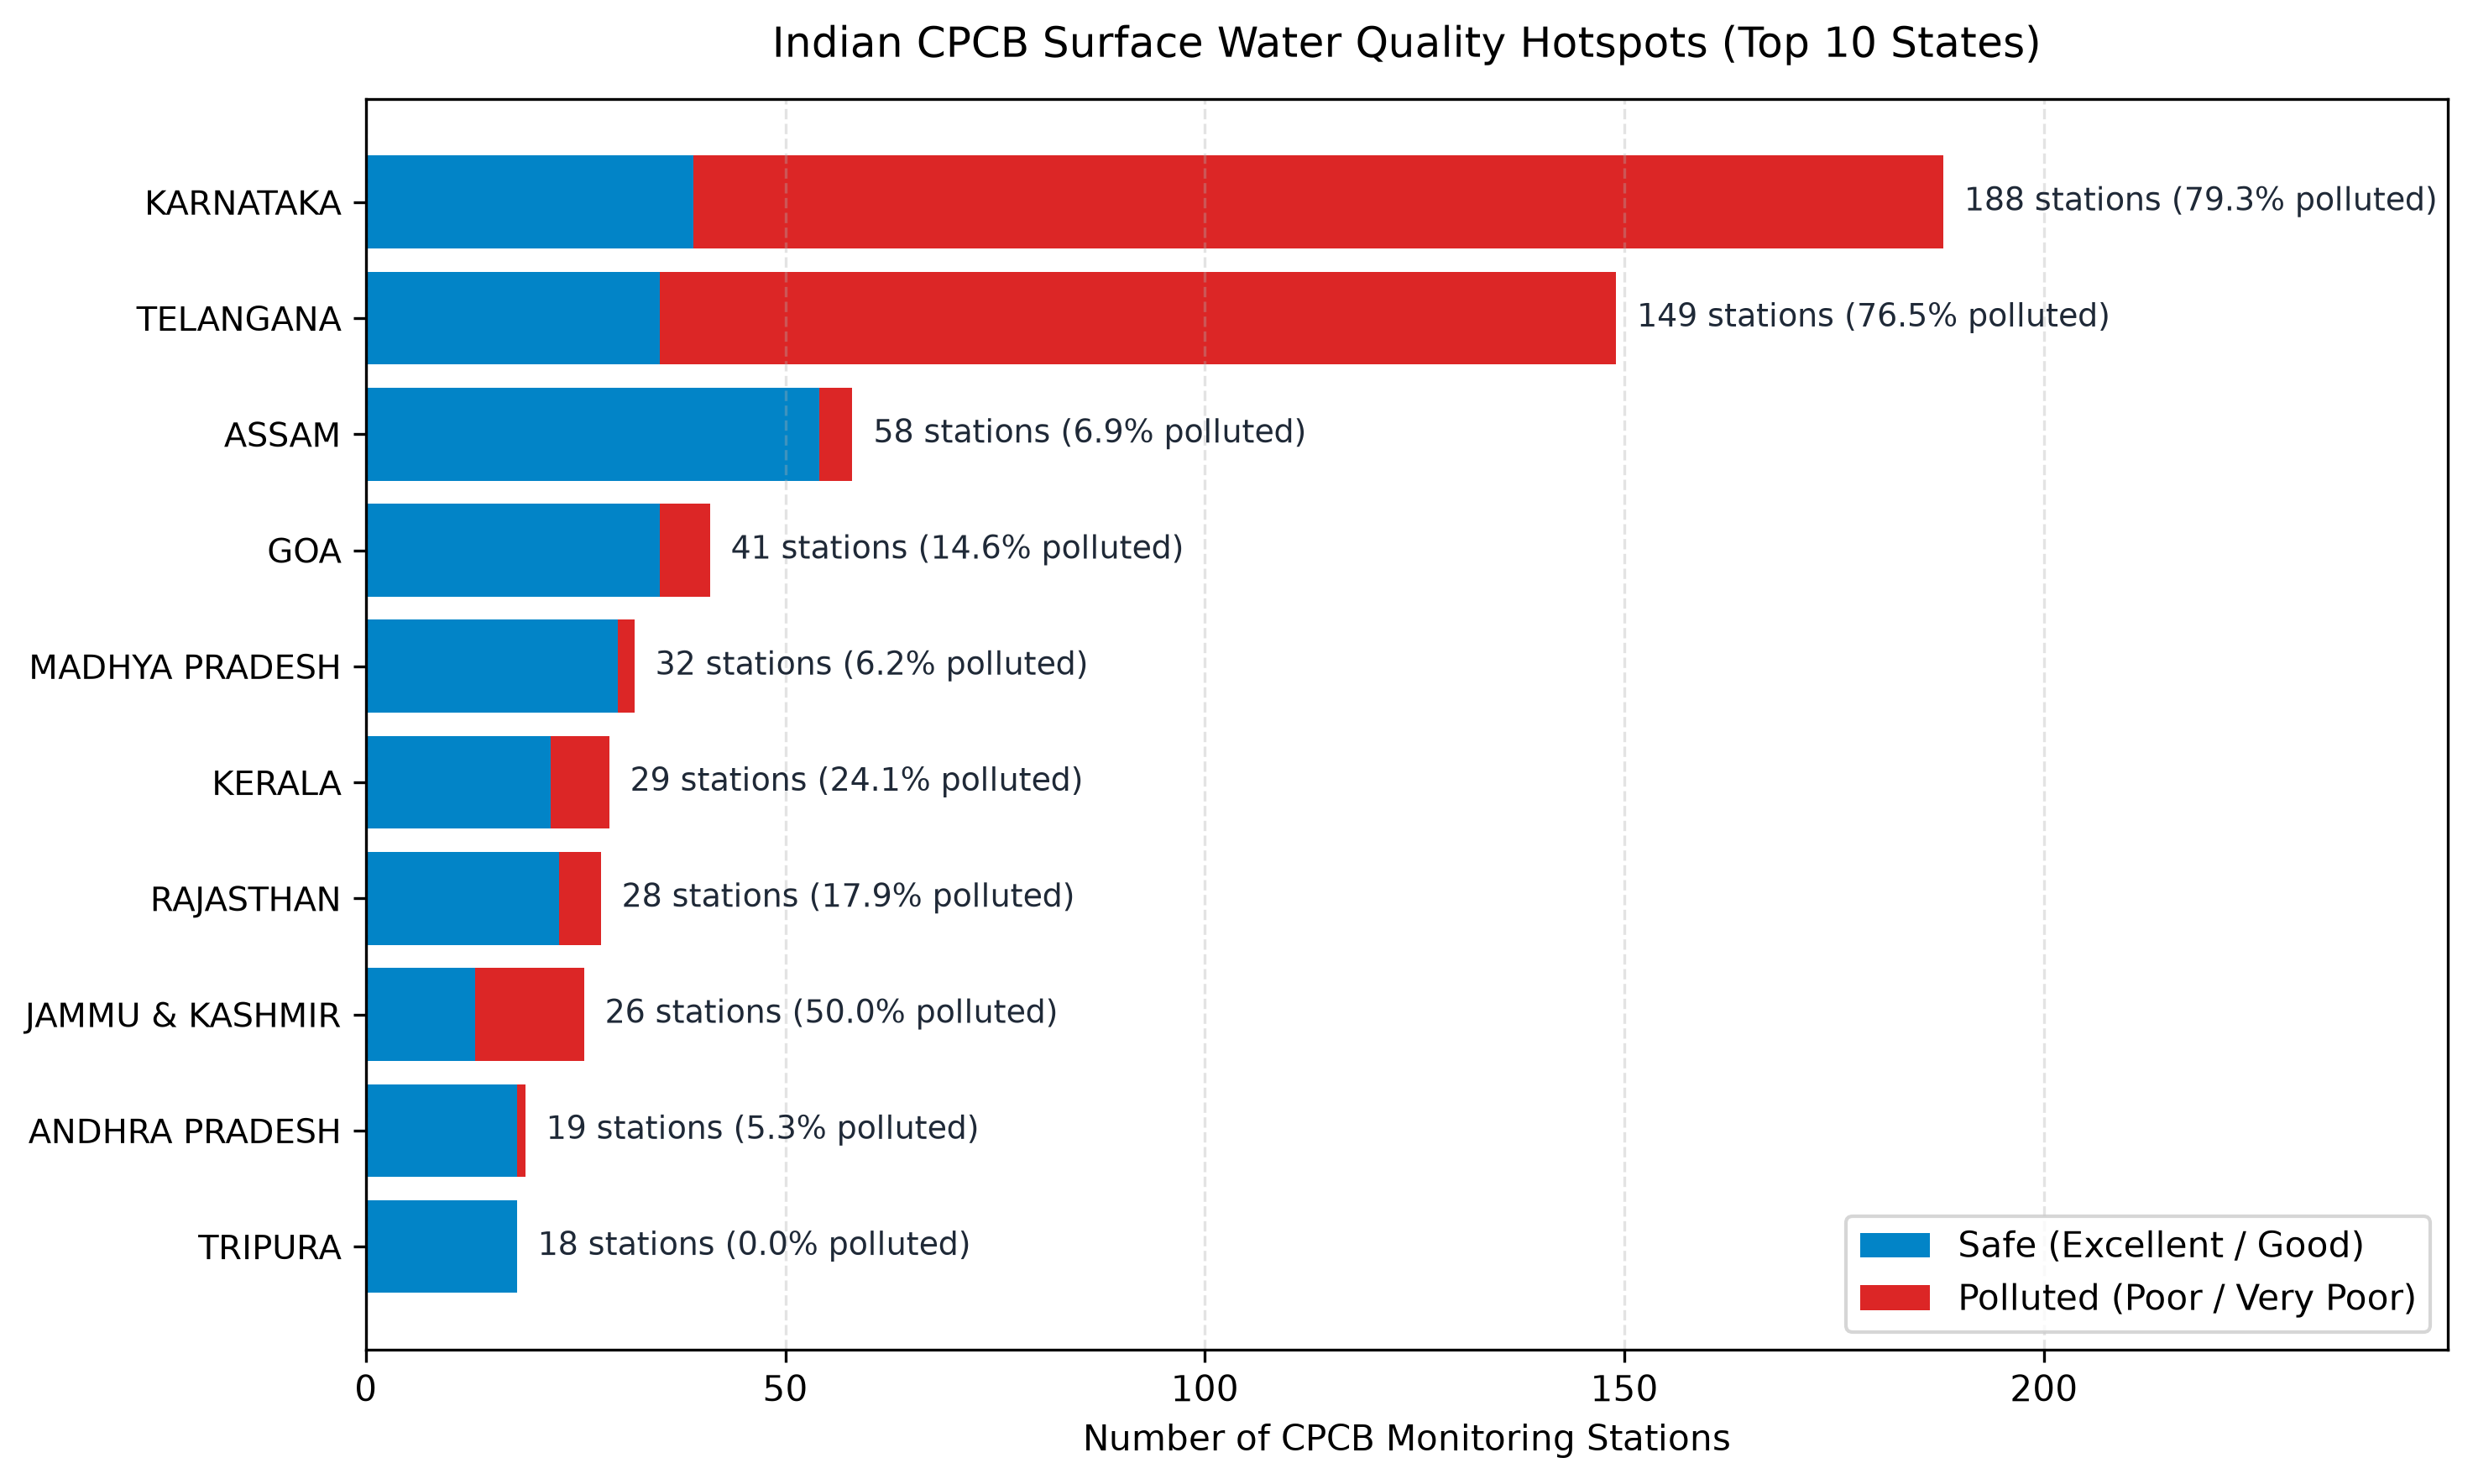
\includegraphics[width=0.86\textwidth]{india_state_pollution.png}
\caption{Geographic distribution of ambient surface-water compliance and degradation across 26 Indian States and Union Territories from the CPCB lentic monitoring network ($N = 683$), illustrating severe spatial clustering.}\label{fig:india_state_pollution}
\end{figure}

On a single stratified test split ($n = 103$), the 18-feature Full Laboratory Suite achieves $98.06\%$ [95\% CI: $93.19\%, 99.47\%$] binary accuracy ($0.9977$ AUC) and $93.20\%$ [$86.63\%, 96.67\%$] 4-class accuracy ($0.9960$ Macro OvR AUC). Because ground-truth CPCB WQI classifications are derived directly from these identical parameters, this high score verifies mathematical formula emulation rather than autonomous ecological discovery.

When restricted to the 11-feature Instant Field-Probe configuration (omitting the 5-day $\text{BOD}_5$ and coliform assays), single-split performance remains high: $92.23\%$ [$85.42\%, 96.01\%$] binary accuracy ($0.9837$ AUC) and $69.90\%$ [$60.46\%, 77.91\%$] 4-class accuracy ($0.9297$ Macro OvR AUC).

\begin{table}[t]
\caption{Identical-fold spatial cross-validation on the Indian CPCB 11-feature Instant Field-Probe ($N = 683$, 26 States).}\label{tab:cpcb_spatial}%
\tiny\setlength{\tabcolsep}{1.5pt}
\begin{tabular*}{\textwidth}{@{\extracolsep\fill}p{0.10\textwidth}p{0.15\textwidth}cccc@{}}
\toprule
Spatial CV Scheme & Model (11 Probe Features) & Pooled OOF Acc [95\% CI] & Fold Mean $\pm$ Std & Pooled F1 / Macro-F1 & Pooled AUC / OvR \\
\midrule
5-Fold \texttt{GroupKFold} & \textbf{Binary RF (11 Probe)} & $\mathbf{0.8726}$ [84.55, 89.56\%] & $0.8778 \pm 0.0317$ & $\mathbf{0.8869}$ & $\mathbf{0.9224}$ \\
5-Fold \texttt{GroupKFold} & Binary Logistic Reg (11 Probe) & $0.8536$ [82.51, 87.81\%] & $0.8515 \pm 0.0368$ & $0.8599$ & $0.8981$ \\
5-Fold \texttt{GroupKFold} & Binary Heuristic ($\text{DO}_{\min} \ge 4.0$) & $\mathbf{0.8785}$ [85.18, 90.09\%] & $0.8697 \pm 0.0653$ & $0.8865$ & --- \\
5-Fold \texttt{GroupKFold} & 4-Class Regularized RF (11 Probe) & $0.4993$ [46.19, 53.67\%] & --- & $0.4835$ & $0.7761$ (OvR) \\
\midrule
Leave-One-State-Out & \textbf{Binary RF (11 Probe)} & $\mathbf{0.8697}$ [84.24, 89.29\%] & $0.8390 \pm 0.2648$ & $\mathbf{0.8840}$ & $\mathbf{0.9177}$ \\
Leave-One-State-Out & Binary Logistic Reg (11 Probe) & $0.8492$ [82.04, 87.41\%] & $0.8196 \pm 0.2680$ & $0.8551$ & $0.8888$ \\
Leave-One-State-Out & Binary Heuristic ($\text{DO}_{\min} \ge 4.0$) & $\mathbf{0.8785}$ [85.18, 90.09\%] & $0.8108 \pm 0.2676$ & $0.8865$ & --- \\
Leave-One-State-Out & 4-Class Regularized RF (11 Probe) & $0.5183$ [48.08, 55.56\%] & --- & $0.5037$ & $0.7820$ (OvR) \\
\botrule
\end{tabular*}
\end{table}

Because stations within the same state share regional administrative and environmental baselines, Table~\ref{tab:cpcb_spatial} reports spatial cross-validation under 5-Fold \texttt{GroupKFold} and 26-State \texttt{LeaveOneGroupOut} (LOSO), adhering to spatial evaluation standards \cite{roberts2017,ploton2020}. Under 5-Fold \texttt{GroupKFold}, fold sizes and class distributions reflect the strong regional imbalance of the monitoring network: Fold~1 holds out Karnataka alone ($n = 188$, $20.7\%$ Acceptable), Fold~2 holds out Telangana alone ($n = 149$, $23.5\%$ Acceptable), and Folds~3--5 each group $8$ smaller states ($n = 116, 115, 115$ with $81.9\%$, $87.0\%$, and $87.0\%$ Acceptable, respectively). Note that in Table~\ref{tab:cpcb_spatial}, Binary RF ($300$ trees) and Logistic Regression ($L_2$-regularized, $1000$ iterations) are evaluated with fixed baseline configurations rather than nested inner-CV tuning.

For binary triage across unseen states, the Binary RF probe achieves $\mathbf{87.26\%}$ [95\% CI: $84.55\%, 89.56\%$] pooled out-of-fold accuracy ($0.9224$ ROC-AUC) under \texttt{GroupKFold} and $\mathbf{86.97\%}$ [$84.24\%, 89.29\%$] ($0.9177$ ROC-AUC; balanced accuracy $0.8654$) under LOSO. It outperforms the linear Logistic Regression probe baseline ($0.8888$--$0.8981$ ROC-AUC; $84.92\%$--$85.36\%$ accuracy; LOSO balanced accuracy $0.8514$), while the deterministic regulatory threshold heuristic ($\text{DO}_{\min} \ge 4.0\text{ mg/L}$) attains slightly higher pooled accuracy ($87.85\%$) and LOSO balanced accuracy ($0.8785$). On pooled LOSO confusion matrices (Degraded $= 0$, Acceptable $= 1$), $\text{DO}_{\min} \ge 4.0$ yields $\text{TN} = 276, \text{FP} = 38, \text{FN} = 45, \text{TP} = 324$ ($87.90\%$ Degraded recall), whereas Binary RF yields $\text{TN} = 255, \text{FP} = 59, \text{FN} = 30, \text{TP} = 339$ ($81.21\%$ Degraded recall, $91.87\%$ Acceptable recall) alongside continuous, rank-ordered risk probabilities ($0.9177$ ROC-AUC).

To diagnose spatial heterogeneity, Table~\ref{tab:cpcb_loso_states} summarizes per-state LOSO performance across all $10$ states with $n \ge 15$ stations. Transfer performance is strong in Telangana ($89.93\%$ Acc, $0.9934$ AUC), Assam ($98.28\%$ Acc, $0.9954$ AUC), Madhya Pradesh ($93.75\%$ Acc, $0.8500$ AUC), and Odisha ($93.33\%$ Acc, $0.9286$ AUC), but degrades in Jammu \& Kashmir ($69.23\%$ Acc, $0.7633$ AUC), Gujarat ($70.59\%$ Acc, $0.7692$ AUC), and Rajasthan ($85.71\%$ Acc, $0.5739$ AUC). Across the remaining $16$ smaller states/UTs ($n \in [1, 13]$), $9$ are single-class (leaving ROC-AUC undefined) and $6$ contain $n \le 3$ stations (e.g., Haryana $0/2$ and Chhattisgarh $0/1$ degraded stations misclassified), which accounts for the large LOSO fold standard deviation ($\pm 0.2648$).

\begin{table}[t]
\caption{Per-state Leave-One-State-Out (LOSO) binary screening performance for states with $n \ge 15$ stations ($11$-feature Instant Field-Probe).}\label{tab:cpcb_loso_states}%
\tiny\setlength{\tabcolsep}{2pt}
\begin{tabular*}{\textwidth}{@{\extracolsep\fill}lcccccc@{}}
\toprule
State ($n$) & Acceptable / Degraded & RF Acc & LR Acc & $\text{DO}_{\min} \ge 4.0$ Acc & RF ROC-AUC \\
\midrule
Karnataka ($188$) & $39 / 149$ & $0.8191$ & $0.8830$ & $\mathbf{0.9043}$ & $0.9380$ \\
Telangana ($149$) & $35 / 114$ & $0.8993$ & $0.8255$ & $\mathbf{0.9732}$ & $0.9934$ \\
Assam ($58$) & $54 / 4$ & $\mathbf{0.9828}$ & $\mathbf{0.9828}$ & $0.8966$ & $0.9954$ \\
Goa ($41$) & $35 / 6$ & $\mathbf{0.8537}$ & $0.6098$ & $0.6341$ & $0.9857$ \\
Madhya Pradesh ($32$) & $30 / 2$ & $\mathbf{0.9375}$ & $\mathbf{0.9375}$ & $\mathbf{0.9375}$ & $0.8500$ \\
Kerala ($29$) & $22 / 7$ & $0.7931$ & $\mathbf{0.8276}$ & $0.6897$ & $0.9221$ \\
Rajasthan ($28$) & $23 / 5$ & $\mathbf{0.8571}$ & $0.7143$ & $0.8214$ & $0.5739$ \\
Jammu \& Kashmir ($26$) & $13 / 13$ & $\mathbf{0.6923}$ & $\mathbf{0.6923}$ & $0.6538$ & $0.7633$ \\
Andhra Pradesh ($19$) & $18 / 1$ & $\mathbf{1.0000}$ & $\mathbf{1.0000}$ & $\mathbf{1.0000}$ & $1.0000$ \\
Tripura ($18$) & $18 / 0$ & $\mathbf{1.0000}$ & $\mathbf{1.0000}$ & $\mathbf{1.0000}$ & --- \\
Gujarat ($17$) & $13 / 4$ & $0.7059$ & $\mathbf{0.7647}$ & $\mathbf{0.7647}$ & $0.7692$ \\
Odisha ($15$) & $14 / 1$ & $\mathbf{0.9333}$ & $0.7333$ & $0.8000$ & $0.9286$ \\
\botrule
\end{tabular*}
\end{table}

Conversely, 4-class multi-tier field-probe accuracy drops precipitously to $\mathbf{49.93\%}$ (\texttt{GroupKFold}) and $\mathbf{51.83\%}$ (LOSO) across unseen states. This demonstrates that instant field probes are effective for \textbf{rapid binary triage} of CPCB-derived WQI status, but cannot differentiate fine WQI tiers without 5-day laboratory coliform and oxygen-demand incubation.

\begin{figure}[h]
\centering
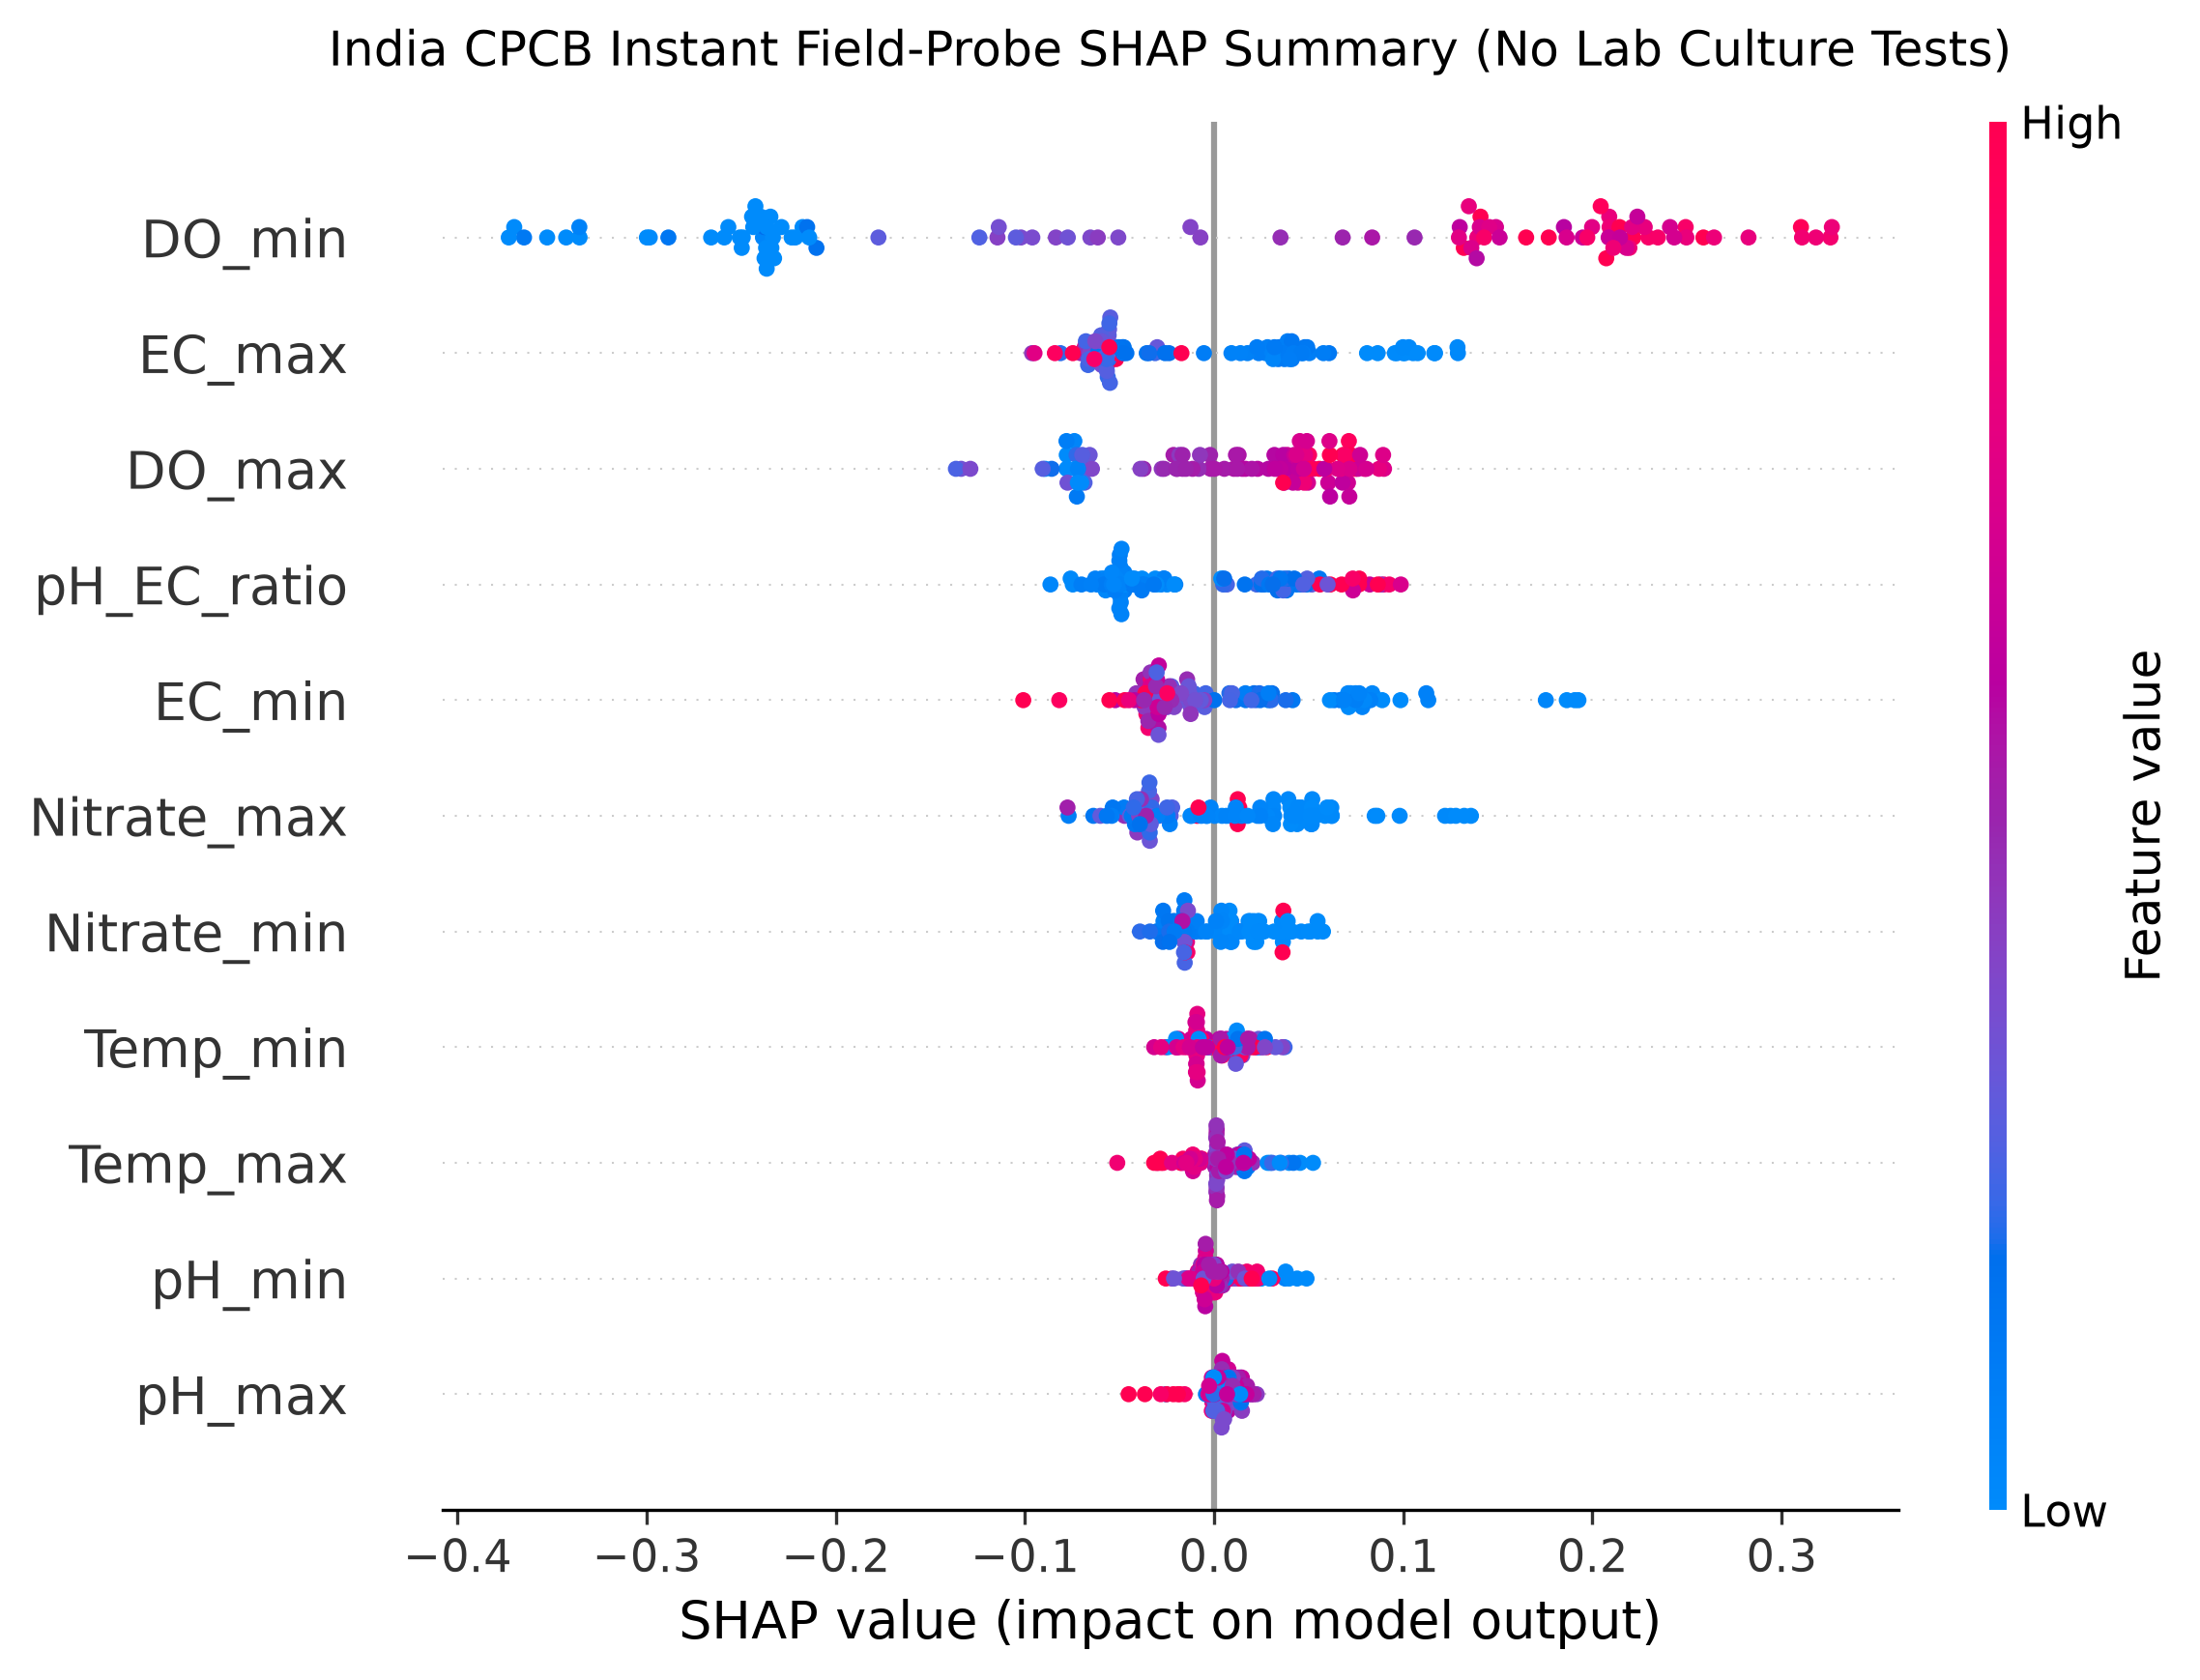
\includegraphics[width=0.76\textwidth]{india_probe_shap_summary.png}
\caption{TreeExplainer SHAP summary plot for the 11-feature Instant Field-Probe model on the Indian CPCB surface-water cohort ($N = 683$), highlighting the predominant predictive influence of minimum dissolved oxygen ($\text{DO}_{\min}$).}\label{fig:india_probe_shap}
\end{figure}

TreeSHAP attribution on the 11-feature field probe (Figure~\ref{fig:india_probe_shap}) indicates that minimum dissolved oxygen dominates feature importance ($\text{mean } |\text{SHAP}| = 0.20585$), followed by electrical conductivity ($\texttt{EC\_max} = 0.05683$), peak aeration ($\texttt{DO\_max} = 0.05196$), and the mineralization ratio ($\texttt{pH\_EC\_ratio} = 0.04765$).


\section{Conclusion and Future Work}\label{sec6}

This study demonstrates that enforcing a strictly leakage-free evaluation protocol reshapes conclusions in water-quality machine learning. On the Kaggle drinking-water benchmark ($N = 3,276$), removing class-conditional imputation leakage eliminates artificial accuracy inflation ($+11.18\%$ on the canonical split; $+12.89 \pm 1.54\%$ across 20 random seeds) and reveals a realistic performance ceiling of $0.68$--$0.71$ ROC-AUC. Under Nadeau--Bengio corrected resampled $t$-tests, RBF SVM, Tuned RF, and Plain RF did not show statistically significant differences ($p \ge 0.2499$), and multivariate ExtraTrees \texttt{IterativeImputer} provided no significant advantage over median imputation ($p = 0.6386$). Moreover, lowering the test False-Safe Rate from $22.67\%$ to $5.00\%$ via a validation-frozen $0.60$ score cutoff requires rejecting $74.48\%$ of genuinely potable water, confirming that routine physicochemical parameters cannot replace microbiological assays for potable water certification.

In the separate Indian CPCB ambient surface-water case study ($N = 683$, 26 States/UTs), 5-fold \texttt{GroupKFold} and 26-state Leave-One-State-Out validation show that 11 instant field-probe parameters achieve $86.97\%$--$87.26\%$ pooled OOF accuracy ($0.9177$--$0.9224$ ROC-AUC) for predicting binary CPCB-derived WQI status without 5-day laboratory $\text{BOD}_5$ or coliform incubation, outperforming linear subset-of-formula Logistic Regression ($0.8888$--$0.8981$ ROC-AUC) while matching the accuracy of a simple $\text{DO}_{\min} \ge 4.0\text{ mg/L}$ threshold heuristic ($87.85\%$). However, 4-class field-probe accuracy drops to $49.93\%$--$51.83\%$ across unseen states, establishing that instant sensors should be restricted to rapid binary triage to prioritize laboratory follow-up.

\paragraph{Limitations and Responsible Deployment}
Several limitations govern the interpretation of these findings. First, the Kaggle drinking-water benchmark lacks microbiological, heavy-metal, and geographic metadata, and cannot independently certify microbiological safety. Second, in the CPCB cohort, state-level grouping tests administrative rather than hydrological watershed independence, and the processed Mendeley v2 release omits sampling dates and frequencies, precluding temporal or seasonal drift evaluation. Third, field-probe deployment in practice is subject to sensor calibration drift and unmeasured contaminants (e.g., pathogens, trace metals, or industrial organics) that do not alter bulk DO, pH, or conductivity. Consequently, neither model is a substitute for statutory laboratory testing or regulatory certification; any operational triage workflow should enforce a human-review and confirmatory laboratory-testing pathway for borderline probabilities, degraded-class alerts, and high-stakes drinking-water decisions. Future work will incorporate microbiological and heavy-metal indicators, evaluate multi-season temporal drift across Indian watersheds, and integrate conformal prediction intervals for distribution-free uncertainty quantification and field abstention \cite{vovk2005,angelopoulos2021}.

\backmatter

\newpage
%%==================================%%
%% 9. References                    %%
%%==================================%%

%% BioMed_Central_Bib_Style_Authyear or sn-mathphys-num

\clearpage
\begin{thebibliography}{65}
\ifx \doiurl \undefined \def \doiurl#1{\url{https://doi.org/#1}}\fi

\bibitem{unesco2023}
UNESCO / UN-Water: The United Nations World Water Development Report 2023: Partnerships and Cooperation for Water.
UNESCO, Paris (2023).

\bibitem{akhtar2021}
Akhtar, N. and Syakir Ishak, M. I. and Bhawani, S. A. and Umar, K.: Various natural and anthropogenic factors responsible for water quality degradation: a review.
\textit{Water} \textbf{13}, 2660 (2021).
\doiurl{10.3390/w13192660}

\bibitem{peters2000}
Peters, N. E. and Meybeck, M.: Water quality degradation effects on freshwater availability: impacts of human activities.
\textit{Water International} \textbf{25}(2), 185--193 (2000).
\doiurl{10.1080/02508060008686817}

\bibitem{rashmi2020}
Rashmi, I. and Roy, T. and Kartika, K. S. and Pal, R. and Coumar, V. and Kala, S. and Shinoji, K. C.: Organic and inorganic fertilizer contaminants in agriculture: impact on soil and water resources.
In: \textit{Contaminants in Agriculture}, pp. 3--41. Springer (2020).
\doiurl{10.1007/978-3-030-41552-5_1}

\bibitem{mccutcheon1992}
McCutcheon, S. C. and Martin, J. L. and Barnwell, T. O.: Water quality.
In: \textit{Handbook of Hydrology}, pp. 11.1--11.73. McGraw-Hill (1992).

\bibitem{who2017}
World Health Organization: Guidelines for Drinking-Water Quality: Fourth Edition Incorporating the First Addendum.
World Health Organization, Geneva (2017).

\bibitem{rachid2025}
Rachid, El-Bacha and Abderrahim, Salhi and Hafid, Abderrafia and Souad, Rabi: Predicting water potability using a machine learning approach.
\textit{Environmental Challenges} \textbf{19}, 101131 (2025).
\doiurl{10.1016/j.envc.2025.101131}

\bibitem{kadiwal2020}
Kadiwal, Aditya: Water Potability Dataset: Cleaned Drinking Water Quality Metrics.
Kaggle Repository, \url{https://www.kaggle.com/datasets/uom190346a/water-potability} (2020).

\bibitem{ghosh2023}
Ghosh, Hritwik and Tusher, M. A. and Rahat, I. S. and Khasim, S. and Mohanty, S. N.: Water quality assessment through predictive machine learning.
In: \textit{Intelligent Computing and Networking (IC-ICN 2023), Lecture Notes in Networks and Systems}, vol. 699. Springer (2023).
\doiurl{10.1007/978-981-99-3177-4_6}

\bibitem{kaddoura2022}
Kaddoura, Sanaa: Evaluation of machine learning algorithm on drinking water quality for better sustainability.
\textit{Sustainability} \textbf{14}(18), 11478 (2022).
\doiurl{10.3390/su141811478}

\bibitem{ahmed2019}
Ahmed, Ali Najah and Othman, Faridah Binti and Afan, Haitham Abdulmohsin and Ibrahim, Ruslan Khalid and Fai, Chow Ming and Hossain, Md. Shahadat and Ehteram, Mohammad and Elshafie, Ahmed: Machine learning methods for better water quality prediction.
\textit{Journal of Hydrology} \textbf{578}, 124084 (2019).
\doiurl{10.1016/j.jhydrol.2019.124084}

\bibitem{bui2020}
Bui, Dieu Tien and Khosravi, Khabat and Tiefenbacher, John and Nguyen, Hoang and Yaseen, Zaher Mundher: Improving forecasting water quality index using novel hybrid machine-learning approach.
\textit{Science of The Total Environment} \textbf{721}, 137612 (2020).
\doiurl{10.1016/j.scitotenv.2020.137612}

\bibitem{aldhyani2020}
Aldhyani, Theyazn H. H. and Al-Yaari, Mohammed and Alkahtani, Hasan and Maashi, Mashael: Water quality prediction using artificial intelligence algorithms.
\textit{Applied Bionics and Biomechanics} \textbf{2020}, 6659314 (2020).
\doiurl{10.1155/2020/6659314}

\bibitem{kaufman2012}
Kaufman, Shachar and Rosset, Saharon and Perlich, Claudia and Stitelman, Ori: Leakage in data mining: Formulation, detection, and avoidance.
\textit{ACM Transactions on Knowledge Discovery from Data (TKDD)} \textbf{6}(4), 1--21 (2012).
\doiurl{10.1145/2382577.2382579}

\bibitem{kapoor2023}
Kapoor, Sayash and Narayanan, Arvind: Leakage and the reproducibility crisis in machine-learning-based science.
\textit{Patterns} \textbf{4}(9), 100804 (2023).
\doiurl{10.1016/j.patter.2023.100804}

\bibitem{legendre1993}
Legendre, Pierre: Spatial autocorrelation: trouble or new paradigm?.
\textit{Ecology} \textbf{74}(6), 1659--1673 (1993).
\doiurl{10.2307/1939924}

\bibitem{roberts2017}
Roberts, David R. and Bahn, Volker and Ciuti, Simone and Boyce, Mark S. and Elith, Jane and Guillera-Arroita, Gurutzeta and Hauenstein, Severin and Lahoz-Monfort, Jos{\'e} J. and Schr{\"o}der, Boris and Thuiller, Wilfried and others: Cross-validation strategies for data with temporal, spatial, hierarchical or phylogenetic structure.
\textit{Ecography} \textbf{40}(8), 913--929 (2017).
\doiurl{10.1111/ecog.02881}

\bibitem{ploton2020}
Ploton, Pierre and Mortier, Fr{\'e}d{\'e}ric and R{\'e}jou-M{\'e}chain, Maxime and Barbier, Nicolas and Picard, Nicolas and Rossi, Vivien and Dormann, Carsten F. and Cornu, Guillaume and Viennois, J{\'e}r{\^o}me and Bayol, Nicolas and others: Spatial validation reveals poor predictive performance of large-scale machine learning models.
\textit{Nature Communications} \textbf{11}(1), 4540 (2020).
\doiurl{10.1038/s41467-020-18321-y}

\bibitem{meyer2018}
Meyer, Hanna and Reudenbach, Christoph and Hengl, Tomislav and Katurji, Marwan and Nauss, Thomas: Improving performance of spatio-temporal machine learning models using spatial cross-validation and feature selection.
\textit{Environmental Modelling \& Software} \textbf{101}, 1--11 (2018).
\doiurl{10.1016/j.envsoft.2017.12.001}

\bibitem{nadeau2003}
Nadeau, Claude and Bengio, Yoshua: Inference for the generalization error.
\textit{Machine Learning} \textbf{52}(3), 239--281 (2003).
\doiurl{10.1023/A:1024068626366}

\bibitem{cpcb2024}
Central Pollution Control Board (CPCB) / NWMP: Processed CPCB-NWMP 2024 Water Quality Dataset and Analysis Code for Explainable Ensemble Classification of Indian Lakes, Ponds, and Tanks (Version 2).
Mendeley Data (CC BY 4.0), \url{https://data.mendeley.com/datasets/6rhkyn9phm/2} (2024).

\bibitem{sokolova2022}
Sokolova, Ekaterina and Ivarsson, O. and Lilliestr{\"o}m, A. and Speicher, N. K. and Rydberg, H. and Bondelind, Mia: Data-driven models for predicting microbial water quality in the drinking water source using \textit{E. coli} monitoring and hydrometeorological data.
\textit{Science of the Total Environment} \textbf{802}, 149798 (2022).
\doiurl{10.1016/j.scitotenv.2021.149798}

\bibitem{mohammed2017}
Mohammed, H. and Hameed, I. A. and Seidu, R.: Random forest tree for predicting fecal indicator organisms in drinking water supply.
In: \textit{2017 International Conference on Behavioral, Economic, Sociocultural Computing (BESC)}, pp. 1--6. IEEE (2017).
\doiurl{10.1109/BESC.2017.8256398}

\bibitem{horton1965}
Horton, Robert K.: An index number system for rating water quality.
\textit{Journal of the Water Pollution Control Federation} \textbf{37}(3), 300--306 (1965).

\bibitem{brown1970}
Brown, Robert M. and McClelland, Nina I. and Deininger, Rolf A. and Tozer, Ronald G.: A water quality index---do we dare?.
\textit{Water \& Sewage Works} \textbf{117}(10), 339--343 (1970).

\bibitem{tyagi2013}
Tyagi, Shweta and Sharma, Bhavtosh and Singh, Prashant and Dobhal, Rajendra: Water quality assessment in terms of water quality index.
\textit{American Journal of Water Resources} \textbf{1}(3), 34--38 (2013).
\doiurl{10.12691/ajwr-1-3-3}

\bibitem{abbasi2012}
Abbasi, Tasneem and Abbasi, S. A.: Water Quality Indices.
Elsevier, Amsterdam (2012).

\bibitem{haghiabi2018}
Haghiabi, Amir Hamzeh and Nasrolahi, Ali Heidar and Parsaie, Abbas: Water quality prediction using machine learning methods.
\textit{Water Quality Research Journal} \textbf{53}(1), 3--13 (2018).
\doiurl{10.2166/wqrj.2018.025}

\bibitem{azrour2022}
Azrour, Mourade and Mabrouki, Jamal and Fattah, G. and Guezzaz, Azidine and Aziz, Faissal: Machine learning algorithms for efficient water quality prediction.
\textit{Modeling Earth Systems and Environment} \textbf{8}, 2793--2801 (2022).
\doiurl{10.1007/s40808-021-01266-6}

\bibitem{ainapure2023}
Ainapure, B. and Baheti, N. and Buch, J. and Appasani, B. and Jha, A. V. and Srinivasulu, A.: Drinking water potability prediction using machine learning approaches: a case study of Indian rivers.
\textit{Water Practice and Technology} \textbf{18}(12), 3004--3020 (2023).
\doiurl{10.2166/wpt.2023.202}

\bibitem{zhu2022}
Zhu, M. and Wang, J. and Yang, X. and Zhang, Y. and Zhang, L. and Ren, H. and Wu, B. and Ye, L.: A review of the application of machine learning in water quality evaluation.
\textit{Eco-Environment \& Health} \textbf{1}(2), 107--116 (2022).
\doiurl{10.1016/j.eehl.2022.06.001}

\bibitem{yan2024}
Yan, X. and Zhang, T. and Du, W. and Meng, Q. and Xu, X. and Zhao, X.: A comprehensive review of machine learning for water quality prediction over the past five years.
\textit{Journal of Marine Science and Engineering} \textbf{12}, 159 (2024).
\doiurl{10.3390/jmse12010159}

\bibitem{rajaee2019}
Rajaee, Taher and Khani, Shima and Ravansalar, Mona: Artificial intelligence-based single and hybrid models for prediction of water quality in rivers: A review.
\textit{Chemometrics and Intelligent Laboratory Systems} \textbf{200}, 103978 (2019).
\doiurl{10.1016/j.chemolab.2020.103978}

\bibitem{vabalas2019}
Vabalas, Andrius and Gowen, Emma and Poliakoff, Ellen and Casson, Alexander J.: Machine learning algorithm validation with a limited sample size.
\textit{PLOS ONE} \textbf{14}(11), e0224365 (2019).
\doiurl{10.1371/journal.pone.0224365}

\bibitem{elkan2001}
Elkan, Charles: The foundations of cost-sensitive learning.
In: \textit{Proceedings of the 17th International Joint Conference on Artificial Intelligence (IJCAI)}, vol. 2, pp. 973--978 (2001).

\bibitem{he2009}
He, Haibo and Garcia, Edwardo A.: Learning from imbalanced data.
\textit{IEEE Transactions on Knowledge and Data Engineering} \textbf{21}(9), 1263--1284 (2009).
\doiurl{10.1109/TKDE.2008.239}

\bibitem{usepa2018}
United States Environmental Protection Agency: 2018 Edition of the Drinking Water Standards and Health Advisories Tables.
Technical Report EPA 822-F-18-001, Office of Water, U.S. EPA (2018).

\bibitem{bis2012}
Bureau of Indian Standards: Indian Standard: Drinking Water---Specification (Second Revision).
Technical Report IS 10500:2012, Bureau of Indian Standards (2012).

\bibitem{pedregosa2011}
Pedregosa, Fabian and Varoquaux, Ga{\"e}l and Gramfort, Alexandre and Michel, Vincent and Thirion, Bertrand and Grisel, Olivier and Blondel, Mathieu and Prettenhofer, Peter and Weiss, Ron and Dubourg, Vincent and others: Scikit-learn: Machine learning in Python.
\textit{Journal of Machine Learning Research} \textbf{12}, 2825--2830 (2011).

\bibitem{vanbuuren2011}
van Buuren, Stef and Groothuis-Oudshoorn, Karin: mice: Multivariate imputation by chained equations in R.
\textit{Journal of Statistical Software} \textbf{45}(3), 1--67 (2011).
\doiurl{10.18637/jss.v045.i03}

\bibitem{little2019}
Little, Roderick J. A. and Rubin, Donald B.: Statistical Analysis with Missing Data.
3rd edn. John Wiley \& Sons, Hoboken, NJ (2019).

\bibitem{breiman2001}
Breiman, Leo: Random forests.
\textit{Machine Learning} \textbf{45}(1), 5--32 (2001).
\doiurl{10.1023/A:1010933404324}

\bibitem{cortes1995}
Cortes, Corinna and Vapnik, Vladimir: Support-vector networks.
\textit{Machine Learning} \textbf{20}(3), 273--297 (1995).
\doiurl{10.1007/BF00994018}

\bibitem{cox1958}
Cox, David R.: The regression analysis of binary sequences.
\textit{Journal of the Royal Statistical Society: Series B (Methodological)} \textbf{20}(2), 215--232 (1958).
\doiurl{10.1111/j.2517-6161.1958.tb00292.x}

\bibitem{liu1989}
Liu, Dong C. and Nocedal, Jorge: On the limited memory BFGS method for large scale optimization.
\textit{Mathematical Programming} \textbf{45}(1--3), 503--528 (1989).
\doiurl{10.1007/BF01589116}

\bibitem{breiman1984}
Breiman, Leo and Friedman, Jerome and Olshen, Richard and Stone, Charles: Classification and Regression Trees.
\textit{} (1984).

\bibitem{cover1967}
Cover, Thomas and Hart, Peter: Nearest neighbor pattern classification.
\textit{IEEE Transactions on Information Theory} \textbf{13}(1), 21--27 (1967).
\doiurl{10.1109/TIT.1967.1053964}

\bibitem{zadrozny2002}
Zadrozny, Bianca and Elkan, Charles: Transforming classifier scores into accurate multiclass probability estimates.
In: \textit{Proceedings of the Eighth ACM SIGKDD International Conference on Knowledge Discovery and Data Mining (KDD)}, pp. 694--699 (2002).
\doiurl{10.1145/775047.775151}

\bibitem{platt1999}
Platt, John: Probabilistic outputs for support vector machines and comparisons to regularized likelihood methods.
In: \textit{Advances in Large Margin Classifiers}, pp. 61--74. MIT Press (1999).

\bibitem{niculescumizil2005}
Niculescu-Mizil, Alexandru and Caruana, Rich: Predicting good probabilities with supervised learning.
In: \textit{Proceedings of the 22nd International Conference on Machine Learning (ICML)}, pp. 625--632 (2005).
\doiurl{10.1145/1102351.1102430}

\bibitem{brier1950}
Brier, Glenn W.: Verification of forecasts expressed in terms of probability.
\textit{Monthly Weather Review} \textbf{78}(1), 1--3 (1950).
\doiurl{10.1175/1520-0493(1950)078<0001:VOFEIT>2.0.CO;2}

\bibitem{lundberg2017}
Lundberg, Scott M. and Lee, Su-In: A unified approach to interpreting model predictions.
In: \textit{Advances in Neural Information Processing Systems (NeurIPS)}, vol. 30, pp. 4765--4774 (2017).

\bibitem{lundberg2020}
Lundberg, Scott M. and Erion, Gabriel and Chen, Hugh and DeGrave, Alex and Prutkin, Jordan M. and Nair, Bala and Katz, Ronit and Himmelfarb, Jonathan and Bansal, Nisha and Lee, Su-In: From local explanations to global understanding with explainable AI for trees.
\textit{Nature Machine Intelligence} \textbf{2}(1), 56--67 (2020).
\doiurl{10.1038/s42256-019-0138-9}

\bibitem{molnar2020}
Molnar, Christoph: Interpretable Machine Learning: A Guide for Making Black Box Models Explainable.
2nd edn. Leanpub (2020).

\bibitem{virtanen2020}
Virtanen, Pauli and Gommers, Ralf and Oliphant, Travis E. and Haberland, Matt and Reddy, Tyler and Cournapeau, David and Burovski, Evgeni and Peterson, Pearu and Weckesser, Warren and Bright, Jonathan and others: SciPy 1.0: Fundamental algorithms for scientific computing in Python.
\textit{Nature Methods} \textbf{17}(3), 261--272 (2020).
\doiurl{10.1038/s41592-019-0686-2}

\bibitem{harris2020}
Harris, Charles R. and Millman, K. Jarrod and van der Walt, St{\'e}fan J. and Gommers, Ralf and Virtanen, Pauli and Cournapeau, David and Wieser, Eric and Taylor, Julian and Berg, Sebastian and Smith, Nathaniel J. and others: Array programming with NumPy.
\textit{Nature} \textbf{585}(7825), 357--362 (2020).
\doiurl{10.1038/s41586-020-2649-2}

\bibitem{mckinney2010}
McKinney, Wes: Data structures for statistical computing in Python.
In: \textit{Proceedings of the 9th Python in Science Conference (SciPy 2010)}, pp. 51--56 (2010).

\bibitem{wilson1927}
Wilson, Edwin B.: Probable inference, the law of population, and the binomial distribution.
\textit{Science} \textbf{65}(1681), 268--270 (1927).
\doiurl{10.1126/science.65.1681.268}

\bibitem{mcnemar1947}
McNemar, Quinn: Note on the sampling error of the difference between correlated proportions or percentages.
\textit{Psychometrika} \textbf{12}(2), 153--157 (1947).
\doiurl{10.1007/BF02295996}

\bibitem{dietterich2000}
Dietterich, Thomas G.: Ensemble methods in machine learning.
In: \textit{Multiple Classifier Systems (MCS 2000), Lecture Notes in Computer Science}, vol. 1857, pp. 1--15. Springer (2000).
\doiurl{10.1007/3-540-45014-9_1}

\bibitem{wolpert1992}
Wolpert, David H.: Stacked generalization.
\textit{Neural Networks} \textbf{5}(2), 241--259 (1992).
\doiurl{10.1016/S0893-6080(05)80023-1}

\bibitem{geurts2006}
Geurts, Pierre and Ernst, Damien and Wehenkel, Louis: Extremely randomized trees.
\textit{Machine Learning} \textbf{63}(1), 3--42 (2006).
\doiurl{10.1007/s10994-006-6226-1}

\bibitem{streamlit2020}
Streamlit Inc.: Streamlit: An Open-Source Python Framework for Data Science and Machine Learning Applications.
\url{https://streamlit.io} (2020).

\bibitem{vovk2005}
Vovk, Vladimir and Gammerman, Alex and Shafer, Glenn: Algorithmic Learning in a Random World.
Springer, New York (2005).
\doiurl{10.1007/b106715}

\bibitem{angelopoulos2021}
Angelopoulos, Anastasios N. and Bates, Stephen: A gentle introduction to conformal prediction and distribution-free uncertainty quantification.
\textit{arXiv preprint arXiv:2107.07511} (2021).

\end{thebibliography}
\section*{Declarations}

\begin{itemize}
\item \textbf{Funding:} The author declares that no external funding was received for this study.
\item \textbf{Conflict of interest/Competing interests:} The author declares no competing financial or non-financial interests.
\item \textbf{Ethics approval and consent to participate:} Not applicable (study uses publicly available secondary environmental datasets).
\item \textbf{Consent for publication:} Not applicable.
\item \textbf{Data availability:} The drinking-water potability dataset is publicly available on Kaggle (\texttt{water\_potability.csv}). The Indian CPCB surface-water dataset is publicly available under a Creative Commons Attribution 4.0 International (CC BY 4.0) licence at Mendeley Data: \textit{Processed CPCB-NWMP 2024 Water Quality Dataset and Analysis Code for Explainable Ensemble Classification of Indian Lakes, Ponds, and Tanks} (v2, 2024), \url{https://data.mendeley.com/datasets/6rhkyn9phm/2}.
\item \textbf{Materials availability:} Not applicable.
\item \textbf{Code availability:} The complete Python source code, leak-free pipeline scripts, and spatial validation workflows will be made publicly available in the project repository upon publication (repository URL and release tag to be inserted in the final version).
\item \textbf{Author contribution:} Conceptualization, methodology, software implementation, validation, formal analysis, and manuscript drafting were performed by the sole author.
\end{itemize}

\end{document}
